%&preformat-disser
\RequirePackage[l2tabu,orthodox]{nag} % Раскомментировав, можно в логе получать рекомендации относительно правильного использования пакетов и предупреждения об устаревших и нерекомендуемых пакетах
% Формат А4, 14pt (ГОСТ Р 7.0.11-2011, 5.3.6)
\documentclass[a4paper,14pt,oneside,openany]{memoir}

%%%%%%%%%%%%%%%%%%%%%%%%%%%%%%%%%%%%%%%%%%%%%%%%%%%%%%%%%%%%%%%%%%%%%%%%%%%%%%%%
%%%% Файл упрощённых настроек шаблона, общих для диссертации и автореферата %%%%
%%%%%%%%%%%%%%%%%%%%%%%%%%%%%%%%%%%%%%%%%%%%%%%%%%%%%%%%%%%%%%%%%%%%%%%%%%%%%%%%

%%% Режим черновика %%%
\makeatletter
\@ifundefined{c@draft}{
  \newcounter{draft}
  \setcounter{draft}{0}  % 0 --- чистовик (максимальное соблюдение ГОСТ)
                         % 1 --- черновик (отклонения от ГОСТ, но быстрая
                         %       сборка итоговых PDF)
}{}
\makeatother

%%% Пометки в тексте %%%
\makeatletter
\@ifundefined{c@showmarkup}{
  \newcounter{showmarkup}
  \setcounter{showmarkup}{0}  % 0 --- скрыть пометки
                              % 1 --- показывать пометки
}{}
\makeatother

%%% Использование в pdflatex шрифтов не по-умолчанию %%%
\makeatletter
\@ifundefined{c@usealtfont}{
  \newcounter{usealtfont}
  \setcounter{usealtfont}{1}    % 0 --- шрифты на базе Computer Modern
                                % 1 --- использовать пакет pscyr, при его
                                %       наличии
                                % 2 --- использовать пакет XCharter, при наличии
                                %       подходящей версии
}{}
\makeatother

%%% Использование в xelatex и lualatex семейств шрифтов %%%
\makeatletter
\@ifundefined{c@fontfamily}{
  \newcounter{fontfamily}
  \setcounter{fontfamily}{1}  % 0 --- CMU семейство. Используется как fallback;
                              % 1 --- Шрифты от MS (Times New Roman и компания)
                              % 2 --- Семейство Liberation
}{}
\makeatother

%%% Библиография %%%
\makeatletter
\@ifundefined{c@bibliosel}{
  \newcounter{bibliosel}
  \setcounter{bibliosel}{1}   % 0 --- встроенная реализация с загрузкой файла
                              %       через движок bibtex8;
                              % 1 --- реализация пакетом biblatex через движок
                              %       biber
}{}
\makeatother

%%% Вывод типов ссылок в библиографии %%%
\makeatletter
\@ifundefined{c@mediadisplay}{
  \newcounter{mediadisplay}
  \setcounter{mediadisplay}{1}   % 0 --- не делать ничего; надписи [Текст] и
                                 %       [Эл. ресурс] будут выводиться только в ссылках с
                                 %       заполненным полем `media`;
                                 % 1 --- автоматически добавлять надпись [Текст] к ссылкам с
                                 %       незаполненным полем `media`; таким образом, у всех
                                 %       источников будет указан тип, что соответствует
                                 %       требованиям ГОСТ
                                 % 2 --- автоматически удалять надписи [Текст], [Эл. Ресурс] и др.;
                                 %       не соответствует ГОСТ
                                 % 3 --- автоматически удалять надпись [Текст];
                                 %       не соответствует ГОСТ
                                 % 4 --- автоматически удалять надпись [Эл. Ресурс];
                                 %       не соответствует ГОСТ
}{}
\makeatother

%%% Предкомпиляция tikz рисунков для ускорения работы %%%
\makeatletter
\@ifundefined{c@imgprecompile}{
  \newcounter{imgprecompile}
  \setcounter{imgprecompile}{0}   % 0 --- без предкомпиляции;
                                  % 1 --- пользоваться предварительно
                                  %       скомпилированными pdf вместо генерации
                                  %       заново из tikz
}{}
\makeatother
            % общие настройки шаблона
\input{common/packages}         % Пакеты общие для диссертации и автореферата
\synopsisfalse                      % Этот документ --- не автореферат
\input{Dissertation/dispackages}    % Пакеты для диссертации
\input{Dissertation/userpackages}   % Пакеты для специфических пользовательских задач

%%%%%%%%%%%%%%%%%%%%%%%%%%%%%%%%%%%%%%%%%%%%%%%%%%%%%%
%%%% Файл упрощённых настроек шаблона диссертации %%%%
%%%%%%%%%%%%%%%%%%%%%%%%%%%%%%%%%%%%%%%%%%%%%%%%%%%%%%

%%% Инициализирование переменных, не трогать!  %%%
\newcounter{intvl}
\newcounter{otstup}
\newcounter{contnumeq}
\newcounter{contnumfig}
\newcounter{contnumtab}
\newcounter{pgnum}
\newcounter{chapstyle}
\newcounter{headingdelim}
\newcounter{headingalign}
\newcounter{headingsize}
%%%%%%%%%%%%%%%%%%%%%%%%%%%%%%%%%%%%%%%%%%%%%%%%%%%%%%

%%% Область упрощённого управления оформлением %%%

%% Интервал между заголовками и между заголовком и текстом %%
% Заголовки отделяют от текста сверху и снизу
% тремя интервалами (ГОСТ Р 7.0.11-2011, 5.3.5)
\setcounter{intvl}{3}               % Коэффициент кратности к размеру шрифта

%% Отступы у заголовков в тексте %%
\setcounter{otstup}{0}              % 0 --- без отступа; 1 --- абзацный отступ

%% Нумерация формул, таблиц и рисунков %%
% Нумерация формул
\setcounter{contnumeq}{0}   % 0 --- пораздельно (во введении подряд,
                            %       без номера раздела);
                            % 1 --- сквозная нумерация по всей диссертации
% Нумерация рисунков
\setcounter{contnumfig}{0}  % 0 --- пораздельно (во введении подряд,
                            %       без номера раздела);
                            % 1 --- сквозная нумерация по всей диссертации
% Нумерация таблиц
\setcounter{contnumtab}{1}  % 0 --- пораздельно (во введении подряд,
                            %       без номера раздела);
                            % 1 --- сквозная нумерация по всей диссертации

%% Оглавление %%
\setcounter{pgnum}{1}       % 0 --- номера страниц никак не обозначены;
                            % 1 --- Стр. над номерами страниц (дважды
                            %       компилировать после изменения настройки)
\settocdepth{subsection}    % до какого уровня подразделов выносить в оглавление
\setsecnumdepth{subsection} % до какого уровня нумеровать подразделы


%% Текст и форматирование заголовков %%
\setcounter{chapstyle}{1}     % 0 --- разделы только под номером;
                              % 1 --- разделы с названием "Глава" перед номером
\setcounter{headingdelim}{1}  % 0 --- номер отделен пропуском в 1em или \quad;
                              % 1 --- номера разделов и приложений отделены
                              %       точкой с пробелом, подразделы пропуском
                              %       без точки;
                              % 2 --- номера разделов, подразделов и приложений
                              %       отделены точкой с пробелом.

%% Выравнивание заголовков в тексте %%
\setcounter{headingalign}{0}  % 0 --- по центру;
                              % 1 --- по левому краю

%% Размеры заголовков в тексте %%
\setcounter{headingsize}{0}   % 0 --- по ГОСТ, все всегда 14 пт;
                              % 1 --- пропорционально изменяющийся размер
                              %       в зависимости от базового шрифта

%% Подпись таблиц %%

% Смещение строк подписи после первой строки
\newcommand{\tabindent}{0cm}

% Тип форматирования заголовка таблицы:
% plain --- название и текст в одной строке
% split --- название и текст в разных строках
\newcommand{\tabformat}{plain}

%%% Настройки форматирования таблицы `plain`

% Выравнивание по центру подписи, состоящей из одной строки:
% true  --- выравнивать
% false --- не выравнивать
\newcommand{\tabsinglecenter}{false}

% Выравнивание подписи таблиц:
% justified   --- выравнивать как обычный текст («по ширине»)
% centering   --- выравнивать по центру
% centerlast  --- выравнивать по центру только последнюю строку
% centerfirst --- выравнивать по центру только первую строку (не рекомендуется)
% raggedleft  --- выравнивать по правому краю
% raggedright --- выравнивать по левому краю
\newcommand{\tabjust}{justified}

% Разделитель записи «Таблица #» и названия таблицы
\newcommand{\tablabelsep}{~\cyrdash\ }

%%% Настройки форматирования таблицы `split`

% Положение названия таблицы:
% \centering   --- выравнивать по центру
% \raggedleft  --- выравнивать по правому краю
% \raggedright --- выравнивать по левому краю
\newcommand{\splitformatlabel}{\raggedleft}

% Положение текста подписи:
% \centering   --- выравнивать по центру
% \raggedleft  --- выравнивать по правому краю
% \raggedright --- выравнивать по левому краю
\newcommand{\splitformattext}{\raggedright}

%% Подпись рисунков %%
%Разделитель записи «Рисунок #» и названия рисунка
\newcommand{\figlabelsep}{~\cyrdash\ }  % (ГОСТ 2.105, 4.3.1)
                                        % "--- здесь не работает

%%% Цвета гиперссылок %%%
% Latex color definitions: http://latexcolor.com/
\definecolor{linkcolor}{rgb}{0.9,0,0}
\definecolor{citecolor}{rgb}{0,0.6,0}
\definecolor{urlcolor}{rgb}{0,0,1}
%\definecolor{linkcolor}{rgb}{0,0,0} %black
%\definecolor{citecolor}{rgb}{0,0,0} %black
%\definecolor{urlcolor}{rgb}{0,0,0} %black

\newtheorem{theorem}{Теорема}
\newtheorem{lemma}{Лемма}
\newcommand{\T}{^\top}
      % Упрощённые настройки шаблона

% Новые переменные, которые могут использоваться во всём проекте
% ГОСТ 7.0.11-2011
% 9.2 Оформление текста автореферата диссертации
% 9.2.1 Общая характеристика работы включает в себя следующие основные структурные
% элементы:
% актуальность темы исследования;
\newcommand{\actualityTXT}{Актуальность темы исследования}
% степень ее разработанности;
\newcommand{\progressTXT}{Степень разработанности темы исследования}
% объект и предмет;
\newcommand{\objectsubjectTXT}{Объект и предмет исследования}
% цели и задачи;
\newcommand{\aimtasksTXT}{Цель и задачи диссертационной работы}
%\newcommand{\tasksTXT}{задачи}
% или чаще используют просто
%\newcommand{\influenceTXT}{Практическая значимость}
% методологию и методы исследования;
\newcommand{\methodsTXT}{Методы исследования}
% положения, выносимые на защиту;
\newcommand{\defpositionsTXT}{Положения, выносимые на~защиту}
% соответствие паспорту специальности.
\newcommand{\complianceTXT}{Соответствие результатов диссертации паспорту научной специальности}
% научную новизну;
\newcommand{\noveltyTXT}{Научная новизна результатов}
% степень достоверности результатов.
\newcommand{\probationTXT}{Достоверность и обоснованность результатов}
% теоретическую и практическую значимость работы;
\newcommand{\influenceTXT}{Теоретическая и практическая значимость}
% апробаця результатов
\newcommand{\reliabilityTXT}{Публикации и апробация результатов}
\newcommand{\publicationsTXT}{Публикации}
\newcommand{\contributionTXT}{Личный вклад автора}


%%% Заголовки библиографии:

% для автореферата:
\newcommand{\bibtitleauthor}{Публикации автора по теме диссертации}

% для стиля библиографии `\insertbiblioauthorgrouped`
\newcommand{\bibtitleauthorvak}{В изданиях из списка ВАК РФ}
\newcommand{\bibtitleauthorscopus}{В изданиях, входящих в международную базу цитирования Scopus}
\newcommand{\bibtitleauthorwos}{В изданиях, входящих в международную базу цитирования Web of Science}
\newcommand{\bibtitleauthorother}{В прочих изданиях}
\newcommand{\bibtitleauthorconf}{В сборниках трудов конференций}
\newcommand{\bibtitleauthorpatent}{Зарегистрированные патенты}
\newcommand{\bibtitleauthorprogram}{Зарегистрированные программы для ЭВМ}

% для стиля библиографии `\insertbiblioauthorimportant`:
\newcommand{\bibtitleauthorimportant}{Наиболее значимые \protect\MakeLowercase\bibtitleauthor}

% для списка литературы в диссертации и списка чужих работ в автореферате:
\newcommand{\bibtitlefull}{Список литературы} % (ГОСТ Р 7.0.11-2011, 4)
         % Новые переменные, для всего проекта

\newcommand{\thesisAuthorLastName}{\fixme{Андронова}}
\newcommand{\thesisAuthorOtherNames}{\fixme{Анастасия Алексеевна}}
\newcommand{\thesisAuthorInitials}{\fixme{А.\,А.}}
\newcommand{\thesisAuthor}             % Диссертация, ФИО автора
{%
	\texorpdfstring{% \texorpdfstring takes two arguments and uses the first for (La)TeX and the second for pdf
		\thesisAuthorLastName~\thesisAuthorOtherNames% так будет отображаться на титульном листе или в тексте, где будет использоваться переменная
	}{%
		\thesisAuthorLastName, \thesisAuthorOtherNames% эта запись для свойств pdf-файла. В таком виде, если pdf будет обработан программами для сбора библиографических сведений, будет правильно представлена фамилия.
	}
}
\newcommand{\thesisAuthorShort}        % Диссертация, ФИО автора инициалами
{\thesisAuthorInitials~\thesisAuthorLastName}
%\newcommand{\thesisUdk}                % Диссертация, УДК
%{\fixme{xxx.xxx}}
\newcommand{\thesisTitle}              % Диссертация, название
{\fixme{Ортогональные методы оптимального робастного управления шагающими роботами с использованием линейных матричных неравенств}}
\newcommand{\thesisSpecialtyNumber}    % Диссертация, специальность, номер
{\fixme{1.2.2}}
\newcommand{\thesisSpecialtyTitle}     % Диссертация, специальность, название (название взято с сайта ВАК для примера)
{\fixme{Математическое моделирование, численные методы и комплексы программ}}
\newcommand{\thesisDegree}             % Диссертация, ученая степень
{\fixme{кандидата физико-математических наук}}
\newcommand{\thesisDegreeShort}        % Диссертация, ученая степень, краткая запись
{\fixme{канд. физ.-мат. наук}}
\newcommand{\thesisCity}               % Диссертация, город написания диссертации
{\fixme{Иннополис}}
\newcommand{\thesisYear}               % Диссертация, год написания диссертации
{\the\year}
\newcommand{\thesisOrganization}       % Диссертация, организация
{\fixme{Автономная некоммерческая организация высшего образования <<Университет Иннополис>>}}
\newcommand{\thesisOrganizationShort}  % Диссертация, краткое название организации для доклада
{\fixme{НазУчДисРаб}}

\newcommand{\thesisInOrganization}     % Диссертация, организация в предложном падеже: Работа выполнена в ...
{\fixme{Автономной некоммерческой организации высшего образования <<Университет Иннополис>>}}

%% \newcommand{\supervisorDead}{}           % Рисовать рамку вокруг фамилии
\newcommand{\supervisorFio}              % Научный руководитель, ФИО
{\fixme{Савин Сергей Игоревич}}
\newcommand{\supervisorRegalia}          % Научный руководитель, регалии
{\fixme{Кандидат технических наук, доцент}}
\newcommand{\supervisorFioShort}         % Научный руководитель, ФИО
{\fixme{С.\,И.~Савин}}
\newcommand{\supervisorRegaliaShort}     % Научный руководитель, регалии
{\fixme{к.~т.~н., доцент}}

\newcommand{\opponentOneFio}           % Оппонент 1, ФИО
{\fixme{Фамилия Имя Отчество}}
\newcommand{\opponentOneRegalia}       % Оппонент 1, регалии
{\fixme{доктор физико-математических наук, профессор}}
\newcommand{\opponentOneJobPlace}      % Оппонент 1, место работы
{\fixme{Не очень длинное название для места работы}}
\newcommand{\opponentOneJobPost}       % Оппонент 1, должность
{\fixme{старший научный сотрудник}}

\newcommand{\opponentTwoFio}           % Оппонент 2, ФИО
{\fixme{Фамилия Имя Отчество}}
\newcommand{\opponentTwoRegalia}       % Оппонент 2, регалии
{\fixme{кандидат физико-математических наук}}
\newcommand{\opponentTwoJobPlace}      % Оппонент 2, место работы
{\fixme{Основное место работы c длинным длинным длинным длинным названием}}
\newcommand{\opponentTwoJobPost}       % Оппонент 2, должность
{\fixme{старший научный сотрудник}}

%% \newcommand{\opponentThreeFio}         % Оппонент 3, ФИО
%% {\fixme{Фамилия Имя Отчество}}
%% \newcommand{\opponentThreeRegalia}     % Оппонент 3, регалии
%% {\fixme{кандидат физико-математических наук}}
%% \newcommand{\opponentThreeJobPlace}    % Оппонент 3, место работы
%% {\fixme{Основное место работы c длинным длинным длинным длинным названием}}
%% \newcommand{\opponentThreeJobPost}     % Оппонент 3, должность
%% {\fixme{старший научный сотрудник}}

\newcommand{\leadingOrganizationTitle} % Ведущая организация, дополнительные строки. Удалить, чтобы не отображать в автореферате
{\fixme{Автономная некоммерческая организация высшего образования <<Университет Иннополис>>}}

\newcommand{\defenseDate}              % Защита, дата
{\fixme{DD mmmmmmmm 2025~г.~в~XX часов}}
\newcommand{\defenseCouncilNumber}     % Защита, номер диссертационного совета
{\fixme{Д\,123.456.78}}
\newcommand{\defenseCouncilTitle}      % Защита, учреждение диссертационного совета
{\fixme{Название учреждения}}
\newcommand{\defenseCouncilAddress}    % Защита, адрес учреждение диссертационного совета
{\fixme{Адрес}}
\newcommand{\defenseCouncilPhone}      % Телефон для справок
{\fixme{+7~(0000)~00-00-00}}

\newcommand{\defenseSecretaryFio}      % Секретарь диссертационного совета, ФИО
{\fixme{Фамилия Имя Отчество}}
\newcommand{\defenseSecretaryRegalia}  % Секретарь диссертационного совета, регалии
{\fixme{д-р~физ.-мат. наук}}            % Для сокращений есть ГОСТы, например: ГОСТ Р 7.0.12-2011 + http://base.garant.ru/179724/#block_30000

\newcommand{\synopsisLibrary}          % Автореферат, название библиотеки
{\fixme{Название библиотеки}}
\newcommand{\synopsisDate}             % Автореферат, дата рассылки
{\fixme{DD mmmmmmmm}\the\year~года}

% To avoid conflict with beamer class use \providecommand
\providecommand{\keywords}%            % Ключевые слова для метаданных PDF диссертации и автореферата
{}             % Основные сведения
\input{common/fonts}            % Определение шрифтов (частичное)
% Общие стили оформления.
% Возможные варианты значений ищите в описании библиотеки beamer
\usetheme[progressbar=frametitle]{metropolis}
%\usecolortheme{whale}

\definecolor{mydarkred}{RGB}{ 71, 0, 0}
\definecolor{mygreen}{HTML}{A9AD9B}
% \usetheme[secheader]{Boadilla}
%\usecolortheme{mydarkred}
\setbeamercolor{frametitle}{bg=mydarkred, fg=white}
\setbeamercolor{progress bar}{bg=mygreen!20, fg=mygreen}
% Размер полей слайдов
\setbeamersize{text margin left=1cm,%
               text margin right=1cm}

% выключение кнопок навигации
\beamertemplatenavigationsymbolsempty

\usepackage{ragged2e}
\justifying

% Размеры шрифтов
\setbeamerfont{title}{size=\large}
\setbeamerfont{subtitle}{size=\small}
\setbeamerfont{author}{size=\normalsize}
\setbeamerfont{institute}{size=\small}
\setbeamerfont{date}{size=\normalsize}
\setbeamerfont{bibliography item}{size=\small}
\setbeamerfont{bibliography entry author}{size=\small}
\setbeamerfont{bibliography entry title}{size=\small}
\setbeamerfont{bibliography entry location}{size=\small}
\setbeamerfont{bibliography entry note}{size=\small}
% Аналогично можно настроить и другие размеры.
% Названия классов элементов можно найти здесь
% http://www.cpt.univ-mrs.fr/~masson/latex/Beamer-appearance-cheat-sheet.pdf

% Цвет элементов
\setbeamercolor{footline}{fg=black}
\setbeamercolor{bibliography item}{fg=black}
\setbeamercolor{bibliography entry author}{fg=black}
\setbeamercolor{bibliography entry title}{fg=black}
\setbeamercolor{bibliography entry location}{fg=black}
\setbeamercolor{bibliography entry note}{fg=black}
% Аналогично можно настроить и другие цвета.
% Названия классов элементов можно найти здесь
% http://www.cpt.univ-mrs.fr/~masson/latex/Beamer-appearance-cheat-sheet.pdf

% Нумеровать список статей
% https://tex.stackexchange.com/a/419506/104425
\setbeamertemplate{bibliography item}{\insertbiblabel}
% или убрать номера
% \setbeamertemplate{bibliography item}{}

% Использовать шрифт с засечками для формул
% https://tex.stackexchange.com/a/34267/104425
\usefonttheme[onlymath]{serif}

% https://tex.stackexchange.com/a/291545/104425
\makeatletter
\def\beamer@framenotesbegin{% at beginning of slide
    \usebeamercolor[fg]{normal text}
    \gdef\beamer@noteitems{}%
    \gdef\beamer@notes{}%
}
\makeatother

% footer презентации
\setbeamertemplate{footline}{
    \leavevmode%
    \hbox{%
        \begin{beamercolorbox}[wd=.333333\paperwidth,ht=2.25ex,dp=1ex,center]{}%
            % И. О. Фамилия, Организация кратко
            \thesisAuthorShort
        \end{beamercolorbox}%
        \begin{beamercolorbox}[wd=.333333\paperwidth,ht=2.25ex,dp=1ex,center]{}%
            % Город, 20XX
            \thesisCity, \thesisYear
        \end{beamercolorbox}%
        \begin{beamercolorbox}[wd=.333333\paperwidth,ht=2.25ex,dp=1ex,right]{}%
            Стр. \insertframenumber{} из \inserttotalframenumber \hspace*{2ex}
        \end{beamercolorbox}}%
    \vskip0pt%
}

% вывод на экран заметок к презентации
\ifnumequal{\value{presnotes}}{0}{}{
    \setbeameroption{show notes}
    \ifnumequal{\value{presnotes}}{2}{
        \setbeameroption{show notes on second screen=\presposition}
    }{}
}
           % Стили общие для диссертации и автореферата
\input{Dissertation/disstyles}  % Стили для диссертации
\input{Dissertation/userstyles} % Стили для специфических пользовательских задач

%%% Библиография. Выбор движка для реализации %%%
% Здесь только проверка установленного ключа. Сама настройка выбора движка
% размещена в common/setup.tex
\ifnumequal{\value{bibliosel}}{0}{%
    \input{biblio/predefined}   % Встроенная реализация с загрузкой файла через движок bibtex8
}{
    \input{biblio/biblatex}     % Реализация пакетом biblatex через движок biber
}

% Вывести информацию о выбранных опциях в лог сборки
\typeout{Selected options:}
\typeout{Draft mode: \arabic{draft}}
\typeout{Font: \arabic{fontfamily}}
\typeout{AltFont: \arabic{usealtfont}}
\typeout{Bibliography backend: \arabic{bibliosel}}
\typeout{Precompile images: \arabic{imgprecompile}}
% Вывести информацию о версиях используемых библиотек в лог сборки
\listfiles

%%% Управление компиляцией отдельных частей диссертации %%%
% Необходимо сначала иметь полностью скомпилированный документ, чтобы все
% промежуточные файлы были в наличии
% Затем, для вывода отдельных частей можно воспользоваться командой \includeonly
% Ниже примеры использования команды:
%
%\includeonly{Dissertation/part2}
%\includeonly{Dissertation/contents,Dissertation/appendix,Dissertation/conclusion}
%
% Если все команды закомментированы, то документ будет выведен в PDF файл полностью

\begin{document}
%%% Переопределение именований типовых разделов
% https://tex.stackexchange.com/a/156050
\gappto\captionsrussian{\input{common/renames}} % for polyglossia and babel
\input{common/renames}
\gappto\captionsrussian{\input{Dissertation/renames}} % for polyglossia and babel
\input{Dissertation/renames}

%%% Структура диссертации (ГОСТ Р 7.0.11-2011, 4)
% Титульный лист (ГОСТ Р 7.0.11-2001, 5.1)
\thispagestyle{empty}
\begin{center}
\thesisOrganization
\end{center}
%
\vspace{0pt plus4fill} %число перед fill = кратность относительно некоторого расстояния fill, кусками которого заполнены пустые места
\IfFileExists{images/logo.pdf}{
  \begin{minipage}[b]{0.5\linewidth}
    \begin{flushleft}
      
\includegraphics[height=1.1cm]{logo}
    \end{flushleft}
  \end{minipage}%
  \begin{minipage}[b]{0.5\linewidth}
    \begin{flushright}
      На правах рукописи\\
%      \textsl {УДК \thesisUdk}
    \end{flushright}
  \end{minipage}
}{
\begin{flushright}
На правах рукописи

%\textsl {УДК \thesisUdk}
\end{flushright}
}
%
\vspace{0pt plus6fill} %число перед fill = кратность относительно некоторого расстояния fill, кусками которого заполнены пустые места
\begin{center}
{\large \thesisAuthor}
\end{center}
%
\vspace{0pt plus1fill} %число перед fill = кратность относительно некоторого расстояния fill, кусками которого заполнены пустые места
\begin{center}
\textbf {\large %\MakeUppercase
\thesisTitle}

\vspace{0pt plus2fill} %число перед fill = кратность относительно некоторого расстояния fill, кусками которого заполнены пустые места
{%\small
Специальность \thesisSpecialtyNumber\ "---

<<\thesisSpecialtyTitle>>
}

\ifdefined\thesisSpecialtyTwoNumber
{%\small
Специальность \thesisSpecialtyTwoNumber\ "---

<<\thesisSpecialtyTwoTitle>>
}
\fi

\vspace{0pt plus2fill} %число перед fill = кратность относительно некоторого расстояния fill, кусками которого заполнены пустые места
Диссертация на соискание учёной степени

\thesisDegree
\end{center}
%
\vspace{0pt plus4fill} %число перед fill = кратность относительно некоторого расстояния fill, кусками которого заполнены пустые места
\begin{flushright}
\ifdefined\supervisorTwoFio
Научные руководители:

\supervisorRegalia

\ifdefined\supervisorDead
\framebox{\supervisorFio}
\else
\supervisorFio
\fi

\supervisorTwoRegalia

\ifdefined\supervisorTwoDead
\framebox{\supervisorTwoFio}
\else
\supervisorTwoFio
\fi
\else
Научный руководитель:

\supervisorRegalia

\ifdefined\supervisorDead
\framebox{\supervisorFio}
\else
\supervisorFio
\fi
\fi

\end{flushright}
%
\vspace{0pt plus4fill} %число перед fill = кратность относительно некоторого расстояния fill, кусками которого заполнены пустые места
{\centering\thesisCity\ "--- \thesisYear\par}
           % Титульный лист
\include{Dissertation/contents}        % Оглавление
\ifnumequal{\value{contnumfig}}{1}{}{\counterwithout{figure}{chapter}}
\ifnumequal{\value{contnumtab}}{1}{}{\counterwithout{table}{chapter}}
\chapter*{Введение}                         % Заголовок
\addcontentsline{toc}{chapter}{Введение}    % Добавляем его в оглавление

\newcommand{\actuality}{\textbf{\actualityTXT}}
\newcommand{\progress}{\textbf{\progressTXT}}
\newcommand{\objectsubject}{\textbf{\objectsubjectTXT}}
\newcommand{\aimtasks}{\textbf{\aimtasksTXT}}
\newcommand{\methods}{\textbf{\methodsTXT}}
\newcommand{\defpositions}{\textbf{\defpositionsTXT}}
\newcommand{\compliances}{\textbf{\complianceTXT}}
\newcommand{\novelty}{\textbf{\noveltyTXT}}
\newcommand{\probation}{\textbf{\probationTXT}}
\newcommand{\influence}{\textbf{\influenceTXT}}
\newcommand{\reliability}{\textbf{\reliabilityTXT}}
\newcommand{\publications}{\textbf{\publicationsTXT}}
\newcommand{\contribution}{\textbf{\contributionTXT}}

{\actuality} 

В последние десятилетия мобильным роботам уделяется большое внимание, поскольку они могут исследовать сложную окружающую среду, космос, участвовать в спасательных операциях, выполнять задачи без участия человека и т.д. Мобильные роботы можно разделить на три категории; колёсные, гусеничные и шагающие. Система передвижения робота --- важнейшая характеристика мобильной конструкции, которая зависит не только от рабочего пространства, но и от таких технических показателей, как манёвренность, управляемость, состояние местности, эффективность и устойчивость. Каждая система имеет свои преимущества и недостатки \cite{zhong2019}.

Преимущества передвижения на ногах зависят от позы, количества ног и их функциональности. К примеру, колёсные и гусеничные роботы могут работать на ровной местности, однако большинство из них не могут работать на захламлённой местности, в сложных и опасных условиях. Шагающий робот обладает большим потенциалом для передвижения практически по всей поверхности земли в различных условиях, как и человек, и животное \cite{Silva2012}. Животные используют свои ноги для быстрого и надёжного передвижения по различным местностям, обладая отличной локомоцией и ловкостью. Чаще всего они передвигаются с высокой скоростью и эффективностью в зависимости от условий окружающей среды.

Управление шагающими роботами находится в центре внимания исследователей уже несколько десятилетий. Шагающая локомоция объединяет дискретные события (приобретение и потеря контакта между роботом и окружающей средой) с непрерывной динамикой, что делает управление такими системами отличным от многих других известных задач управления. Дискретная природа шагающего движения часто явно закладывается в задаче планирования траектории \cite{katayama2022whole, lu2023whole}, а также в методах управления с прогнозирующими моделями, разработанных для шагающих роботов \cite{KIM2019, chignoli2021humanoid}. Даже когда задача управления формулируется для очень короткого временного горизонта (или одного момента времени), тот факт, что движение включает дискретные шаги, меняет и ограничивает предположения, которые мы можем сделать о модели робота.

Аналитические модели роботов часто бывают неточными и вызывают неопределённость в динамике. Сложный набор датчиков и несколько уровней программного обеспечения вносят шум и задержки в передачу информации. Обычные законы управления часто оказываются недостаточными для эффективного решения этих проблем. Специализированные методы управления, разработанные для решения этой сложной задачи, обычно требуют длительного процесса проектирования и сложной настройки параметров. 

Разработка робастного управления для шагающих роботов является важным направлением в современной робототехнике. Хотя было предложено множество эффективных способов разработки робастных регуляторов для линейных \cite{POLYAK2021, Nicolett2018} и нелинейных \cite{HAUSWIRTH2024, Celentano2018} систем, новые типы роботов ставят новые, часто более сложные версии проблемы робастного управления. Для мобильных роботов не всегда доступно хорошее описание окружающей среды. Кроме того, для шагающих роботов представление их динамики в виде обыкновенного дифференциального уравнения (ОДУ) хорошо работает только на коротких временных горизонтах, например, между последовательными шагами. В результате разработка робастного управления для этого типа роботов приобретает особую форму, которая ранее не рассматривалась в литературе. В данной работе мы решаем задачу робастного управления с комбинацией аддитивных и мультипликативных неопределённостей, связанную с шагающими роботами.

Изменение контакта между роботом и окружающей средой приводит к изменению ограничений, накладываемых на динамику робота. В связи с этим мы можем выбрать описание состояния робота в максимальных координатах, которые состоят из активных состояний, способных изменяться, и статических состояний, вынужденных оставаться постоянными из-за действия ограничений \cite{SAVIN2021}. Влияние статических состояний на модель сродни постоянным внешним силам, действующим на систему. Однако они наследуют структуру от моделей робота и окружающей среды, что может быть использовано при проектировании управления. С другой стороны, они меняются при каждом изменении контакта, что делает многие из известных методов управления, которые работают для статических внешних сил, неприменимыми в данном случае.

Оценка состояния необходима, когда значения некоторых переменных состояния, требуемых законом управления не доступны непосредственно из измерений. Это может быть результатом отсутствия датчиков, шума измерений или выбранной параметризации системы. В типичном сценарии закон управления требует полной информации о состоянии, в то время как только некоторые переменные состояния непосредственно измеряются \cite{Ackermann2001}.

Чтобы учесть такую неопределённость, мы сначала придумаем модель неопределённости, состоящую из модели, которая гарантированно содержит неопределённость системы, и с ней легче работать, а затем спроектировать систему управления, которая удовлетворяет требованиям по устойчивости для всех других возможных моделей в модели неопределённости.

В данной работе мы предлагаем методы проектирования робастного управления и наблюдателей, которые автоматически доказывают устойчивость линеаризованной модели. В то время как существует ряд работ по проектированию управления и наблюдателей для шагающих роботов с точной информацией о модели, вопросы проектирования робастного управления (при мультипликативной неопределённости в модели) в литературе не рассматривались. Также в отличие от существующих методов робастного управления общего назначения, мы одновременно рассматриваем структурированные мультипликативные и аддитивные неопределённости модели.
Методы на основе ортогонального разложения были разработаны для уменьшения размерности вычислений Шуром и другими.

{\progress}

История линейных матричных неравенств в рамках анализа динамических систем начинается с теории Ляпунова. Он показал, что дифференциальное уравнение
\begin{align*}
	\frac{\partial}{\partial t}x(t)=Ax(t)
\end{align*}
устойчиво тогда и только тогда, когда существует положительно определённая матрица $P$ такая, что
\begin{align*}
	A^T P + P A <0.
\end{align*}

Следующее важное развитие теории было сделано в 1940-х годах Лурье \cite{LMI1}, Постниковым и другими. 
Они применили методы Ляпунова к практическим задачам техники управления и вывели линейные матричные неравенства, которые решались аналитически вручную, что ограничивало их применение. 

Следующим важным открытием стало то, что мы сейчас называем леммой о положительно-вещественных матрицах. Она была выведена Калманом, Якубовичем и Поповым в начале 1960-х годов. Им удалось свести решение линейных матричных неравенств, возникающих в задаче Лурье, к простым графическим критериям. Их вклад в \cite{LMI2} заключался в указании способа решения определённого семейства линейных матричных неравенств графическими методами.

Пятницкий и Скородинский \cite{LMI3} были теми, кто сформулировал поиск функции Ляпунова как выпуклую оптимизационную задачу, а затем применили алгоритм, гарантированно решающий её.
В последние десятилетия использование линейных матричных неравенств для проектирования различных регуляторов становится все более популярным. Различные методы \cite{LMI4, LMI5} были объединены с линейными матричными неравенствами, чтобы упростить проектирование регуляторов и продемонстрировать устойчивость управляемой системы.

В последние годы были сделаны различные предложения по достижению робастной устойчивости \cite{LMI7, LMI8}, но их разработка может потребовать больших вычислительных затрат.
Устойчивость по конечному времени также может быть достигнута с помощью линейных матричных неравенств, результаты, представленные в работе \cite{LMI6}, используются для работы с поведением динамических линейных систем «вход-выход». В книге \cite{Amato2011} в едином ключе представлены задачи конечной устойчивости линейных систем, решаемые с помощью линейных матричных неравенств.

Другим способом оценки возмущений, поступающих извне системы, является применение наблюдателя возмущений. Его основная задача --- оценить возмущение на входном этапе, которое затем может быть использовано для борьбы с внешним возмущением. Базовая конструкция регулятора не имеет ограничений, пока она стабилизирует систему при включении наблюдателя возмущений во внутренний контур обратной связи.

Были разработаны различные теоретические методы построения наблюдателей возмущений, большинство из которых рассмотрены в обзорах \cite{ObserverITMO} и \cite{Disturb_obs}. Но в данной работе предлагается использовать наблюдатель для работы с явными механическими ограничениями в виде низкоразмерного наблюдателя состояния, основанного на ортогональных проекциях. Вдохновением для этого послужили работы \cite{SAVIN2021, Righetti2011}, где ортогональные проекции были использованы для замены дифференциальных алгебраических уравнений (ДАУ) для описания динамики эквивалентным ОДУ. 

В линейно--квадратичном регуляторе оптимальный коэффициент усиления регулятора с обратной связью по состоянию может быть получен с помощью алгебраических уравнений Риккати, которые впоследствии используются при проектировании наблюдателя. В работах \cite{LQR1} и \cite{LQR2} был разработан регулятор на основе наблюдателя с использованием линейно--квадратичного регулятора для систем с различными возмущениями. Этот подход широко применим к классу задач оптимального управления со структурными ограничениями. 

{\objectsubject} 

Объектом исследования является оптимальное робастное управление шагающими роботами с мультипликативными и аддитивными неопределённостями, полученными при линеаризации динамической системы.

Предметом исследования являются методы формулирования линейных матричных неравенств для нахождения коэффициентов регулятора и наблюдателя с последующими численными вычислениями для модели шагающего робота.

{\aimtasks} 

Целью диссертационной работы является разработка ортогональных методов оптимального робастного управления шагающими роботами с использованием матричных неравенств.

Для~достижения поставленной цели необходимо было решить следующие задачи:
\begin{enumerate}[beginpenalty=10000] % https://tex.stackexchange.com/a/476052/104425
	\item анализ текущих методов робастного управления для шагающих роботов, вариантов формулирования математической модели для описания движения шагающего робота, способов задания неопределённостей в модели;
	\item разработка метода нахождения оптимального робастного управления для системы с мультипликативными неопределённостями, описывающую шагающего робота;
	\item разработка метода нахождения оптимального робастного управления для системы с мультипликативными и аддитивными неопределённостями, описывающую шагающего робота;
	\item разработка метода нахождения оптимального робастного управления для системы с аддитивными неопределённостями и динамическим управлением, описывающую шагающего робота;
	\item численный анализ разработанных линейных матричных неравенств для нахождения коэффициентов регулятора и наблюдателя для робастного управления, решение прямой задачи динамики, исследование зависимостей результатов от параметров оптимизации;
	\item подтверждение верность разработанных методов на математической модели шагающего робота.
\end{enumerate}

{\methods} 

Для решения вышеуказанных задач и достижения цели использовались методы теории управления и устойчивости, дифференциальных уравнений, численные-аналитические, выпуклой оптимизации, методы математического моделирования, эмпирические данные.

{\defpositions}

\begin{enumerate}[beginpenalty=10000] % https://tex.stackexchange.com/a/476052/104425
	\item метод нахождения оптимального робастного управления для системы с мультипликативными неопределённостями и обратной связью по полному состоянию. Позволяет находить оптимальные коэффициенты регулятора для различных неопределённостей, удовлетворяющих заданным условиям и с использованием линейных матричных неравенств; 
	\item метод нахождения оптимального робастного управления для системы с аддитивными неопределённостями и с динамической обратной связью. Позволяет находить оптимальные коэффициенты регулятора для различных неопределённостей, удовлетворяющих заданным условиям и с использованием линейных матричных неравенств; 
	\item метод численного анализа для проведения численных экспериментов и анализ их результатов, которые верифицировали предыдущие положения.
\end{enumerate}

{\compliances} 

Содержание диссертации соответствует пунктам паспорта научной специальности 1.2.2 --- «Математическое моделирование, численные методы и комплексы программ» (физико--математические науки).
\begin{enumerate}[beginpenalty=10000]
	\item математическое моделирование
	\item численные методы
	\item комплексы программ
\end{enumerate}

{\novelty}

Основные результаты, полученные в работе, являются новыми. В частности
\begin{enumerate}[beginpenalty=10000] % https://tex.stackexchange.com/a/476052/104425
	\item впервые разработаны методы робастного оптимального управления с обратной связью по полному состоянию, используя линейные матричные неравенства для систем с механическими ограничениями и неопределённостями;
	\item впервые разработаны методы робастного оптимального управления с динамической обратной связью, используя линейные матричные неравенства для систем с механическими ограничениями и неопределённостями;
	\item было проведено оригинальное исследование модели шагающего робота, её ортогональной декомпозиции и линеаризации перед разработкой оптимального робастного управления.
\end{enumerate}

{\probation}

Достоверность полученных результатов обеспечивается строгими математическими доказательствами теоретических результатов, корректностью исходных и упрощающих допущений для численного вычисления, адекватными результатами вычислительных экспериментов, использованием уравнений, методов и подходов, строго обоснованных в научной литературе, апробированы и хорошо зарекомендованных при разработке робастного управления для систем с неопределённостями. 

{\influence} 

Теоретическая значимость состоит в разработке нового метода для вычисления коэффициентов регулятора и наблюдателя для робастного управления системы с мультипликативными неопределённостями с использованием линейных матричных неравенств.

Практическая значимость результатов подтверждается применением результатов теоретической части в практике: приводятся формулировки оптимизационных проблем для поиска коэффициентов регуляторов и наблюдателей для управления динамических систем, описывающих динамику шагающего робота. 

{\reliability} 

Результаты, включённые в данную работу, опубликованы в 2 печатных изданиях, 1 из которых изданы в журналах, рекомендованных ВАК, 1 --- в периодических научных журналах, индексируемых \textit{Web of Science} и \textit{Scopus}. 

Результаты находятся в соответствии с результатами, полученными другими авторами. Результаты работы неоднократно докладывались на научно--методических семинарах и были использованы в учебной программе Университета Иннополис.

{\contribution} 

Все результаты, выносимые на защиту, получены лично автором: выбор методик решения задач, разработка алгоритма построения оптимального робастного управления, написание программ для моделирования шагающих роботов и использования разработанных численных экспериментов и анализ результатов расчётов. Постановка задач, обсуждение и интерпретация полученных результатов осуществлялась совместно с научным руководителем. % Характеристика работы по структуре во введении и в автореферате не отличается (ГОСТ Р 7.0.11, пункты 5.3.1 и 9.2.1), потому её загружаем из одного и того же внешнего файла, предварительно задав форму выделения некоторым параметрам

\textbf{Объем и структура работы} 

Диссертация состоит из~введения,
\formbytotal{totalchapter}{глав}{ы}{}{},
заключения и
\formbytotal{totalappendix}{приложен}{ия}{ий}{}.
%% на случай ошибок оставляю исходный кусок на месте, закомментированным
%Полный объём диссертации составляет  \ref*{TotPages}~страницу
%с~\totalfigures{}~рисунками и~\totaltables{}~таблицами. Список литературы
%содержит \total{citenum}~наименований.
%
Полный объём диссертации составляет
\formbytotal{TotPages}{страниц}{у}{ы}{}, включая
\formbytotal{totalcount@figure}{рисун}{ок}{ка}{ков} и
\formbytotal{totalcount@table}{таблиц}{у}{ы}{}.
Список литературы содержит
\formbytotal{citenum}{наименован}{ие}{ия}{ий}.

Во введении приводятся обоснование актуальности темы исследования, степень разработанности темы исследования, формулируются объект и предмет исследования, цель, задачи, научная новизна, методы исследования, положения, выносимые на защиту, описываются теоретическая и практическая значимость работы, внедрение результатов, степень достоверности полученных результатов; приводятся сведения об апробации работы и личном вкладе автора.

В первой главе проведён литературный обзор по теме исследования. Изучены особенности шагающих роботов, а также методы построения управления для них. Исследованы причины для ортогональной декомпозиции и различные методы для её применения. Подняты вопросы робастного управления, в том числе для шагающих роботов. Исследована мультипликативная неопределённости в модели. Приведены методы основанные на линейных матричных неравенствах для робастного управления. Описаны используемые математические инструменты.

Во второй главе приведено описание шагающих роботов и их особенностей на примере четырёхногих роботов. Показан алгоритм линеаризации динамической модели и неопределённостей.

В третей главе представлены результаты разработки оптимизационной проблемы для поиска коэффициентов регулятора и наблюдателя для системы с мультипликативной неопределённостью. Приведены результаты разработки алгоритма для поиска коэффициентов регулятора по обратной связи.

В четвёртой главе диссертационной работы представлены результаты исследования численных методов приведённых в предыдущей главе и проведены численные эксперименты на модели четвероногого робота.

В заключении перечислены результаты работы и направления дальнейших исследований.    % Введение
\ifnumequal{\value{contnumfig}}{1}{\counterwithout{figure}{chapter}
}{\counterwithin{figure}{chapter}}
\ifnumequal{\value{contnumtab}}{1}{\counterwithout{table}{chapter}
}{\counterwithin{table}{chapter}}
\chapter{Обзор литературы}\label{ch:ch1}
\nomenclature{ОДУ}{Обыкновенное дифференциальное уравнение}
\nomenclature{ДАУ}{Дифференциальное алгебраическое уравнение}
\section{Шагающие роботы}\label{sec:ch1/sec1}

Шагающие роботы предлагают больше возможностей по сравнению с колёсными и гусеничными роботами с точки зрения условий работы. Шагающие роботы могут передвигаться по обычной и неровной местности без каких-либо аппаратных изменений и демонстрируют исключительную мобильность \cite{Silva2012}. Колёсные транспортные средства требуют для передвижения асфальтированных (или хотя бы сглаженных) поверхностей, но при этом они чрезвычайно быстры и эффективны на них. Также колёсные механизмы в большинстве случаев являются лёгкими и простыми в конструировании и использовании \cite{Zen2006}. Однако более 50 процентов поверхности Земли недоступно для традиционных транспортных средств, и колёсным машинам трудно или даже невозможно справиться с большими препятствиями и неровностями поверхности. Вездеходы могут преодолевать лишь небольшие препятствия и неровности, но только за счёт высокого потребления энергии \cite{Bekker1962}. Что касается гусеничных машин, то, хотя они и обеспечивают повышенную мобильность на сложных участках, они не в состоянии преодолеть многие препятствия, а их энергопотребление относительно велико. К этим проблемам следует добавить тот факт, что традиционные транспортные средства оставляют на земле сплошные колеи, что в некоторых ситуациях неприменимо, например, с экологической точки зрения. 

Из всего вышесказанного можно сделать вывод, что системы передвижения на ногах обеспечивают лучшую мобильность на естественных участках местности, поскольку эти транспортные средства могут использовать отдельные опоры для каждой ноги, в отличие от колёсных транспортных средств, которым необходима непрерывная опорная поверхность. Шагающие роботы могут передвигаться по неровной местности, изменяя конфигурацию ног, чтобы адаптироваться к неровностям поверхности, и, кроме того, ноги могут устанавливать контакт с землёй в отдельных точках в соответствии с условиями местности. Когда транспортные средства передвигаются по мягким поверхностям, например, по песчаной почве, возможность использовать дискретные опоры в грунте может также улучшить энергопотребление, поскольку они деформируют рельеф меньше, чем колёсные или гусеничные транспортные средства \cite{Iida2007}. 

Энергия, необходимая для выхода из углублений шагающему роботу, меньше \cite{Bekker1962, bekker1969}, а площадь контакта стопы с землёй может быть такой, чтобы давление на опору было небольшим. Кроме того, использование нескольких степеней свободы в суставах ног позволяет шагающим роботам менять направление движения без проскальзывания. Также можно варьировать высоту корпуса, создавая эффект демпфирования и развязки между неровностями рельефа и кузовом транспортного средства (и, как следствие, его полезной нагрузкой). Что касается движения, то следует также упомянуть о возможности, которую предоставляют эти системы, прижиматься к местности, по которой они движутся. Это особенно верно, если они перемещаются, например, по внешней поверхности труб, чтобы повысить способность к балансировке \cite{Kaneko2002}.

Четвероногие роботы --- лучший выбор среди всех ножных роботов с точки зрения мобильности и стабильности управления. Четыре ноги робота легко контролируются, проектируются и обслуживаются по сравнению с двумя или шестью ногами. Биологически вдохновлённая локомоция беговой походки способна выдержать большую полезную нагрузку и балансировку четвероногого робота. Для достижения скорости в реальном времени и естественного движения, как у коровы, собаки, гепарда, необходима разработанная система управления и динамическая генерация походки четвероногих роботов \cite{gonccalves2013}.

Четырёхногие роботы вдохновлены локомоцией четвероногих животных: шарнирные соединения в коленях, бёдрах и шее позволяют им повторять их движения. Самый ранний пример такого робота датируется 1870 годом, когда Чебышев сконструировал четвероногий механизм, который мог стоять и ходить, но не мог адаптироваться к местности \cite{Cheb1948}. В 1893 году Рюгг получил первый патент на ножную машину --- симулятор верховой езды, приводимый в движение педалями \cite{patent}. Заметный шаг в развитии четвероногих роботов произошёл в 1940 году, когда Хатчинсон сконструировал автономно управляемого робота на ногах, подчёркивая преимущества педальных систем перед колёсными или гусеничными машинами для работы с тяжёлыми грузами \cite{Hutchinson1967}.  Кульминацией этого подхода стала постройка компанией \textit{Bucyrus--Eire} в 1969 году самой большой машины на ногах \textit{Big Muskie} \cite{haddock2001extreme}. Этот массивный робот проработал в открытых карьерах 22 года, продемонстрировав целесообразность использования четвероногих механизмов для крупномасштабных промышленных применений.

В 1980-х годах профессор Хиросэ из Токийского технологического института создал семейство четвероногих роботов, ключевой вехой которого стал \textit{PV-II}. Этот робот оснащён моторизованным приводом для каждой ноги, что позволяет ему эффективно ходить \cite{Hirose2009}. Дальнейшие разработки, такие как четвероногий робот \textit{OSQ} из Стэнфорда, продвинули понимание галопирующей походки и энергоэффективного передвижения \cite{Nichol2004}.  Совсем недавно китайские институты, такие как Шаньдунский университет, разработали четвероногих роботов \textit{SCalf--1} и \textit{SCalf--2}, оснащённых усовершенствованными гидравлическими системами для улучшения адаптации к местности и повышения скорости \cite{Rong2012}.

Несмотря на все потенциальные преимущества шагающих роботов, на текущем этапе развития есть несколько аспектов, которые необходимо улучшить и оптимизировать. Одним из недостатков является сложность законов управления. В большинстве случаев, среди всех необходимых вычислений, требуются обратные матрицы инерции жёсткого тела в нескольких местах, что делает этот подход чувствительным к ошибкам моделирования и оценки параметров \cite{Nakanishi_IJRR_2008}. 

\section{Управление для шагающих роботов}\label{sec:ch1/sec2}

Управление подвижными шагающими роботами представляет собой сложную задачу из--за недостаточной динамики тела во время шагов и из--за ограничений, накладываемых на силы реакции на грунт. Исследования в основном были сосредоточены на определении положения и ориентации основания, а также каждой ноги, при рассмотрении системы четвероногих роботов как плавающей в пространстве системы с несколькими телами. Переменные состояния включают в себя конфигурацию тела и углы сочленения ног. Управляющие силы в системе включают крутящие моменты в суставах и силы реакции на грунт.

Желаемая траектория движения тела и каждой ноги может быть сформирована с помощью предварительного планирования или включение ограничений. Помимо ограничений, связанных с контактом с землёй и трением, задачи могут быть описаны в виде уравнений или неравенств, включающих переменные состояния или моменты вращения суставов. Чтобы решить проблему противоречивых ограничений задачи, необходимо использовать соответствующие уравнения оптимизации при проектировании иерархического управления. Такой иерархический регулятор, известный как регулятор всего тела \cite{fahmi2019passive}, объединяет задачи для всех систем робота. 

Планирование и управление движением занимают центральное место в работе четвероногих роботов, включая формирование и выполнение походки. К распространённым методам формирования походки относятся генераторы центрального паттерна, модель перевёрнутого маятника с пружинной нагрузкой, метод нулевой точки момента и траектории кривых Безье.

Модельное прогнозирующее управление --- это метод итеративного решения проблем оптимизации на основе режимов, учитывающий текущее состояние системы и прогнозирующий его изменение в будущем \cite{KIM2019}. Использование управления с прогнозирующими моделями повышает универсальность локомоции, позволяя переключаться между различными походками, просто меняя последовательность контактов. Однако использование управления с прогнозирующими моделями с простой моделью имеет фундаментальное ограничение в управлении положением из--за низкой частоты обновления и упрощения модели. 

В последнее время в научной литературе наблюдается растущий интерес к оптимизационным методам планирования траекторий и управления шагающими роботами. Это связано с высокой эффективностью этих методов, их способностью учитывать различные ограничения, иерархию задач, механические связи и другие факторы. Появление высокопроизводительных вычислителей и эффективных алгоритмов для решения задач выпуклого программирования открыло новые возможности для применения таких методов управления. Существует значительное разнообразие разработанных методов оптимизационного управления, которое не имеет чёткой систематизации. Кроме того, отсутствуют методологии для анализа устойчивости и робастности этих систем управления, а также интегрированные подходы к планированию последовательностей шагов и выбору управляющих воздействий.

Выпуклая оптимизация позволяет обойтись без методов нелинейной оптимизации, которые, в отличие от решателей выпуклой оптимизации, не гарантируют нахождения глобального оптимума и могут страдать от численных проблем \cite{boyd2004convex}. Стабилизация четвероногого робота \textit{HyQ} с помощью выпуклой оптимизации, рассмотренная в \cite{Focchi2016}, демонстрирует практичность выпуклой оптимизации, но этот подход не может быть немедленно распространён на динамические походки из-за  упрощений, внесённых в модель робота.

\section{Ортогональные методы}\label{sec:ch1/sec3}

Существует целый ряд работ по проектированию управления для очень большого класса систем, описываемых ДАУ или вырожденными ОДУ, называемых дескрипторными системами. В этой области исследований есть результаты по робастному управлению и проектированию наблюдателей \cite{Cheng2018, Darouach2014}. Однако методы, разработанные в этой области, недостаточны для решения проблемы, рассматриваемой в данном диссертационном исследовании. В работе \cite{Aghili2003} была предложена процедура для моделирования механических систем с явными ограничениями, что устанавливает связь с более ранними работами в области численных методов для ДАУ, такими как \cite{Liang1987} и другие, в которых рассматривалась очень похожая проблема. 

Для дескрипторных систем с неопределённостями были разработаны методы построения законов управления, например \cite{LIN19993319, Darouach2014}. Однако, при работе с ДАУ и введением в систему неопределённостей возникает необходимость допущений, например введение условия на структуру и ранг дифференциальной матрицы \cite{Cheng2017}, сложность точных вычислений для больших размерностей \cite{Zhang2006}. Результаты представленные в данной работе в сравнение с результатами теории дескрипторных систем заключается в систематическом способе получения низкоразмерного наблюдателя состояния на основе ортогональных проекций, который можно рассматривать как автоматическое восстановление минимального представления статической компоненты на дескрипторе состояния. 

Методы управления системами, предложенные в данной работе, основаны на ортогональных проекциях. Существует ряд существующих методов, основанных на ортогональных проекциях и декомпозиции, разработанных для систем с явными ограничениями, которые мы рассмотрим в этом подразделе. Результаты, наиболее близкие к предлагаемому в данной работе, можно найти в работах, посвящённых управлению механическими системами с явными ограничениями, поэтому мы сосредоточим наше обсуждение на них.

В работах \cite{Aghili2003, Aghili2005}, а также в более поздних работах \cite{Mistry2010, Righetti2011, Righetti2013} были использованы ортогональные проекции. В \cite{Aghili2003, Aghili2005} был предложен ряд новых эквивалентных моделей в неминимальных координатах, в то время как в \cite{Mistry2010, Righetti2011, Righetti2013}, следуя более ранним исследованиям \cite{Khatib2007, Sentis2005}, основное внимание было уделено разработке закона управления. Однако, как было показано в \cite{Righetti2011}, ряд независимо разработанных проекционных методов управления даёт одинаковые (вплоть до разрешения избыточности момента) законы управления.

Для облегчения дизайна и вычислений управления для систем с неопределённостями при помощи линейных матричных неравенств, систему необходимо сначала линеаризовать. Линеаризовать динамику шагающего робота можно, взяв линейный член разложения Тейлора его нелинейной модели. Проецируя его динамику на касательное пространство к множеству ограничений (множество допустимых состояний при текущем контакте с окружающей средой), мы получаем линейную стационарную модель, которая может быть использована, например, для проектирования линейно--квадратичного регулятора \cite{mason2014full}. Однако при этом не учитывается эффект статических состояний, о котором говорилось ранее.

Выделение статических состояний и рассмотрение их как постоянной составляющей динамики позволяет спроектировать наблюдатель состояния как для активных, так и для статических состояний, как это было сделано в \cite{SAVIN2021}. Этот подход все ещё ограничен случаями, когда мультипликативная неопределённость отсутствует. В данной работе мы предлагаем метод, способный работать как со статическими состояниями, так и с мультипликативной неопределённостью.

\section{Робастное управление}\label{sec:ch1/sec4}
Все аналитические методы проектирования управления основаны на «модели» управляемой системы. Такая модель не обязательно представляет собой идеальное описание системы по нескольким причинам, например:
\begin{enumerate}[beginpenalty=10000]
	\item Сложность реальной физической системы не может быть полностью отражена в математических моделях, даже в том случае, когда для данной системы может быть разработана идеальная модель, в общем случае эта модель не будет являться идеальным описанием при всех условиях эксплуатации;
	\item Экспериментальное подтверждение модели системы (включая доказательство достоверности математической модели) очень сложна для нестабильных механизмов \cite{Oral2022};
	\item Даже для стабильных установок очень трудно получить точное экспериментальное измерение высокочастотного поведения;
	\item Некоторые характеристики модели могут не поддаваться «простому» проектированию управления (например, нелинейность, очень высокий порядок ДАУ или быстрая динамика). В этих случаях может оказаться предпочтительным сформулировать простую линейную модель системы, которая может быть использована в качестве основы для проектирования управления \cite{barmish1994new, Garulli2000}.
\end{enumerate}

Тем не менее, даже если идеальная модель системы недоступна, желательно разработать систему автоматического управления, которая будет работать в соответствии с некоторыми спецификациями не только для данной «модели», но и для «реальной» системы.

В робототехнике связанной с шагающими роботами к робастной устойчивости подходили с разных сторон, включая стратегии восстановления после толчка \cite{Pratt2006}, разработку управления с прогнозирующими моделями со свойствами робастной устойчивости \cite{KIM2019} и т.д. Несмотря на то, что были достигнуты значительные результаты в плане производительности роботов, не хватало методов с формальными гарантиями робастности. Прямое применение линейных методов управления к управлению шагающими роботами было затруднено из-за свойств динамики таких роботов, которые приводят к другому типу линейных моделей, о чем будет рассказано в следующем подразделе.

Кроме того, ограничения вводят замкнутые кинематические цепи, делая системы чрезмерно управляемыми \cite{Furieri2017}, с другой стороны, в отсутствие ограничений такие системы, как шагающие роботы с плавающей базой, являются недостаточно управляемыми и неконтролируемыми. Это создаёт дополнительные проблемы с оценкой состояния, поскольку некоторые состояния в координатах плавающей базы не наблюдаются и не влияют на динамику системы. 

Более того, структура динамики механических систем приводит к тому, что одни и те же переменные появляются как в состоянии, так и в его производной по времени (это происходит с обобщёнными скоростями в динамике Лагранжа или уравнениями манипулятора, когда они выражаются в форме пространства состояний). Эта информация может быть потеряна, если ограничения накладываются только на производные состояния, как это было сделано в \cite{Mason2017}, если она учитывается, это дополнительно упрощает задачу оценки состояния.

В целом, одним из наиболее распространённых подходов является использование расширенного фильтра Калмана для оценки состояния робота, использующего информацию о походке и ожидаемом характере контактного взаимодействия со средой, а также кинематическую структуру робота, делая при этом некоторые предположения об упомянутых контактных взаимодействиях и наличии конкретных датчиков \cite{Bloesch2012, Teng2021}. Эти методы были успешно использованы для ножных роботов в ряде экспериментов и практических задач.

По отношению к методу, предлагаемому в данной работе, мы можем рассматривать их как эффективное использование специфических для платформы свойств для построения высокоэффективного оценщика, в то время как предлагаемый метод имеет преимущество общего характера, потенциально требуя меньше работы для адаптации к новой платформе. Эта связь аналогична той, что существует между линейно--квадратичными регуляторами и специфическими для платформы алгоритмами управления с прогнозирующими моделями, разработанными для конкретных типов ножных роботов.

\section{Робастность и мультипликативная неопределённость в модели}\label{sec:ch1/sec5}

Неопределённость в системах может быть учтена двумя основными способами \cite{Radek2017}. Либо можно использовать модель с параметрической неопределённостью \cite{barmish1994new, Bhattacharyya2009}, структура которой фиксирована, но параметры предполагаются лежащими в заданных пределах, либо модель с неструктурированной неопределённостью \cite{Doyle2009, Kucera2007}, где может использоваться даже неизвестный порядок для определения неопределённости. Оба метода имеют свои преимущества и недостатки. Параметрическая неопределённость кажется более естественной и относительно простой для понимания, в то время как преимуществом неструктурированной неопределённости обычно является более лёгкое применение сложных методов проектирования регуляторов. В качестве альтернативы в \cite{Tan2003} изучается совокупность параметрической и неструктурированной неопределённости.

В данной работе рассматривается один из видов неструктурированной неопределённости, известный как мультипликативная неопределённость. Мультипликативная неопределённость может возникать из взаимодействия различных случайных факторов, и занимает центральное место в современных исследованиях. Например, в некоторых случаях шум является мультипликативным, а не аддитивным, и предположение о гауссовости неадекватно из-за природы процесса \cite{Bosse2016, Panza2015}.

Современные подходы к интеграции робастных методов и мультипликативной неопределённости открывают новые горизонты для разработки более эффективных алгоритмов управления. В \cite{Radek2017} рассматриваются различные стратегии, направленные на улучшение устойчивости роботизированных систем при наличии неопределённости. Авторы предлагают комплексный подход, включающий как теоретические, так и практические аспекты, что позволяет создать более надёжные и адаптивные модели роботов. Эти исследования подчёркивают необходимость дальнейшего изучения взаимодействия между робастностью и мультипликативной неопределённостью для достижения высоких показателей эффективности в робототехнике.

Основная цель исследований, связанных с неопределённостями --- предоставить подход к построению модели мультипликативной неопределённости на основе системы с реальной параметрической неопределённостью, а также изобразить методику анализа устойчивости \cite{Skogestad2005}.

В работе \cite{Mabrouk2023}, авторы моделировали неопределённость как аддитивную, возникающую в датчиках или исполнительных механизмах. Основным недостатком похожих методов является то, что они рассматривают неисправности датчиков и исполнительных механизмов как аддитивные. Тем не менее, некоторые ошибки в приводах и датчиках, в дополнение к ошибкам компонентов, часто встречаются в мультипликативной форме. В результате мультипликативные ошибки и входы и выходы системы смешиваются. Поэтому при обобщении методов, рассматривающихся в данной работе, для моделирования системы будут предложены как и мультипликативные так и аддитивные неопределённости.
 
\section{Ближайшие аналоги}\label{sec:ch1/sec6}

Методы, основанные на линейных матричных неравенствах, были ранее предложены для проектирования робастных регуляторов для линейных стационарных систем с нормированными мультипликативными неопределённостями \cite{POLYAK2021,ROTONDO2014}. Однако, неопределённость в данных работах сформулирована не во всех матрицах системы.

При конструировании линейных матричных неравенств для того, чтобы их можно было потом посчитать численно, необходимо достичь линейности в переменных. Использование теории Ляпунова для одновременного проектирования линейного регулятора и наблюдателя Люенбергера для линейной стационарной системы приводит к оптимизационным задачам с ограничениями в виде билинейных матричных неравенств. В \cite{LIEN2004} эта проблема решается путём добавления дополнительного условия для преобразования задачи к линейному матричному неравенству, там авторы рассматривали неопределённости как в матрице состояния, так и в матрице управления линейной стационарной системы. 

В \cite{KHELOUFI2013} авторы использовали неравенство Юнга для преодоления проблемы билинейности, и их метод также учитывает неопределённости как в матрице состояния, так и в матрице наблюдения. В работе \cite{ZEMOUCHE2015} предложен двухшаговый алгоритм для решения проблемы ограничений билинейных матричных неравенств и неопределённостей в матрицах состояния и наблюдения. Неравенство Юнга было использовано для облегчения проектирования управления на основе наблюдателей, а также для работы с мультипликативными неопределённостями, связанными с нормой. В качестве альтернативы, в \cite{GRITLI2021} авторы предлагают метод линейных матричных неравенств для работы с неопределённостями в матрицах состояния, управления и наблюдения, основанный на двух оригинальных леммах, однако численные трудности, связанные с поиском сетки по значению свободного параметра, оказываются одинаковыми во всех приведённых методах.

Одновременное проектирование регулятора и наблюдателя решается как серия задач линейных матричных неравенств \cite{ZEMOUCHE2015,GRITLI2021}. Были предложены $H_\infty$ методы проектирования регуляторов и наблюдателей для линейных стационарных систем с $L_2$ нормированными аддитивными неопределённостями \cite{Bennani2019, KHELOUFI2016}.

На рисунке \ref{fig:table} представлена диаграмма, сортирующая вышеупомянутые методы по типам моделей систем, которые они используют (с ортогональной декомпозицией и в дескрипторной форме), и по типу обратной связи, которую они реализуют: полная обратная связь по состоянию (статическая обратная связь) и динамическая обратная связь по выходу (в форме Люенбергера и в общей форме). Методы, обозначенные ранее были предложены в предыдущей работе \fixme{ссылка на магистерский диплом}.

\begin{figure}[ht]
	\centerfloat{
		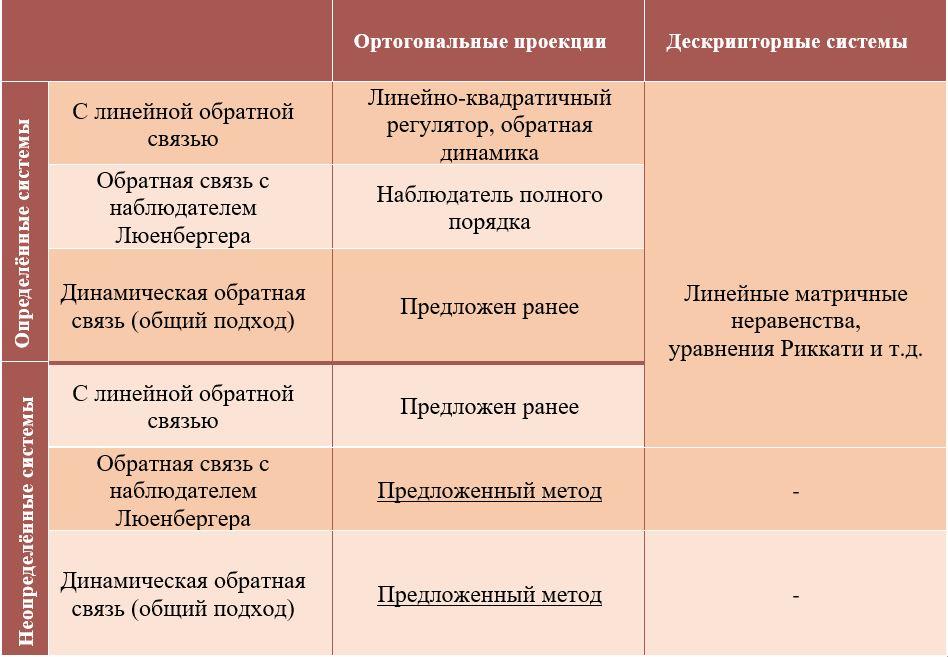
\includegraphics[scale=0.9]{images/table.JPG}
	}
	\caption{Диаграмма методов управления и оценки состояния для систем с явными ограничениями.}\label{fig:table}
\end{figure}

\section{Используемые математические инструменты}\label{sec:ch1/sec7}
В данной работе мы используем неравенство Юнга для решения проблемы билинейности; неопределённости в матрицах моделей также обрабатываются с помощью неравенства Юнга и S--процедуры.

Неравенство Юнга \cite{BOYED1994}, а также S--процедура \cite{Amato2011,LIEN2008} способствуют возникновению свободных скалярных параметров, которые могут внести нелинейность в задачу, особенно когда в ограничениях присутствует как переменная, так и ее инверсия. Решение этой проблемы было описано в \cite{KHELOUFI2016}, где один положительный скаляр и его инверсия были заменены двумя независимыми положительными скалярами. Другая проблема возникает, когда эти скалярные параметры вводят билинейность в задачу. Для этого случая, в \cite{KHELOUFI2013} был предложен метод решетчатого поиска, позволяющий превратить одну билинейную задачу в серию выпуклых задач с ограничениями в виде линейных матричных неравенств.

Дополнение Шура впервые было описано в \cite{Schur} для доказательства леммы Шура. В данной работе дополнение используется для преобразования суммы блочных матриц в одну блочную матрицу для линеаризации переменных в линейных матричных неравенствах.
\FloatBarrier
           % Глава 1
\chapter{Метод математического моделирования для построения управления шагающих роботов}\label{ch:ch2}

\section{Математический метод описания модели и механики контакта}\label{sec:ch2/sect2}
Для построения математической модели робота необходимо учесть механику контакта робота с окружающей средой.
Одним из способов описания контакта является метод, используемый для описания движения с помощью уравнений Лагранжа. В дополнение к классическим формулировкам задач с граничными условиями механики сплошной среды, в контактных задачах вводятся специальные граничные условия, которые управляют движением граничных поверхностей и потенциальных сингулярностей. Для классических контактных задач эти условия выражают ограничение на отсутствие проникновения, закон действия и реакции Ньютона и закон поверхностного трения. Нормальные проекции этих условий предотвращают взаимное проникновение несмешивающихся сред, а тангенциальные проекции учитывают силы трения между соприкасающимися поверхностями \cite{Shamim2024}.

Рассмотрим односторонний точечный контакт --- ограничение ${r}({q}) = 0$, где ${r} \in \mathbb{R}^3$, с соответствующим якобианом ограничений ${J} = \frac{\partial {r}}{\partial {q}}$ и силой реакции ${f} \in \mathbb{R}^3$ \cite{Posa2014}.
%
Сила реакции лежит в конусе трения ${f} \in \mathcal{C}$, с нормальным направлением ${n}$ и коэффициентом трения $\mu$.
%
Такой контакт (ограничение) называется односторонним, потому что связанная с ним сила реакции может «давить», но не «тянуть» на поверхность опоры.

В методах Лагранжа граничные скорости между жёсткими и деформируемыми телами либо задаются, либо корректируются на основе проникновения узлов сетки в запрещённые области, представляющие жёсткие тела. Нормальные компоненты скорости и смещения корректируются для предотвращения проникновения. Если во время коррекции прикладываются внешние нормальные нагрузки, можно определить контактное давление, а трение обрабатывается аналогично другим алгоритмам контакта.

\section{Манипуляторные уравнения для описания динамики шагающих роботов}\label{sec:ch2/sect3}

Рассмотрим уравнение Лагранжа:
%
\begin{equation}
	\frac{d}{dt} \bigg( 
	\frac{\partial T }{\partial \dot{{q}}}
	\bigg) - 
	\frac{\partial T }{\partial {q}} = \tau,
\end{equation}
%
где $T$ --- кинетическая энергия, ${q}$ --- вектор обобщённых координат, а $\tau$ --- обобщённые крутящие моменты. Заметим, что кинетическая энергия может быть описана как $T = \frac{1}{2} \dot{{q}}\T {H} \dot{{q}}$, где ${H}$ --- обобщённая матрица инерции. Матрица ${H}$ является симметричной, положительно определённой и полного ранга.

Обобщённые силы $\tau$ могут быть сформированы декартовыми силами или декартовыми крутящими моментами. Опишем соотношения между декартовой силой ${f}$ и связанной с ней обобщённой силой:

\begin{equation}
	\label{eq:part2_tau}
	\tau_i = \left( \frac{\partial {r}_i}{\partial {q}} \right)\T {f}_i,
\end{equation}
%
где ${r}_i = {r}_i({q})$ --- вектор, описывающий положение точки приложения силы ${f}_i$, как функцию обобщённых координат ${q}$.

При определении якобиана как ${J}_i = \frac{\partial {r}_i}{\partial {q}}$, соотношение \eqref{eq:part2_tau} будет выглядеть как:
%
\begin{equation}
	\tau_i = ({J}^r_i)\T {f}_i.
\end{equation}
%
Соотношение между моментом ${m}$ и связанной с ним обобщённой силой:

\begin{equation}
	\label{eq:part2_tau_j}
	\tau_i = \left( \frac{\partial \omega_i}{\partial \dot{{q}}} \right)\T {m}_i,
\end{equation}
%
где $\omega_i = \omega_i({q}, \dot{{q}})$ --- угловая скорость тела, к которому приложен момент ${m}$.
Определяя якобиан как ${J}^\omega_i = \frac{\partial \omega_i}{\partial \dot{{q}}}$, выражение \eqref{eq:part2_tau_j} принимает вид:
%
\begin{equation}
\tau_i = ({J}^\omega_i)\T {m}_i.
\end{equation}
Определим крутящий момент как ${w} = \begin{bmatrix}
	{f} \\\ {m}
\end{bmatrix}$ и выразим обобщённую силу:
%
\begin{equation}
	\tau_i = \begin{bmatrix}
		{J}^r_i \\\ {J}^\omega_i
	\end{bmatrix}\T
	{w}_i
	=
	{J}_i\T {w}_i.
\end{equation}
Заметим, что полная обобщённая сила может быть вычислена как:
%
\begin{equation}
	\tau = \sum {J}_i\T {w}_i.
\end{equation}
%
Уравнения Лагранжа с ограничениями имеют вид:
%
\begin{equation}
	\begin{cases}
		\frac{d}{dt} \bigg( 
		\frac{\partial T }{\partial \dot{{q}}}
		\bigg) - 
		\frac{\partial T }{\partial {q}} = \tau + \left( \frac{\partial {r}}{\partial {q}} \right)\T \lambda,
		\\
		{r}({q}) = 0,
	\end{cases}
\end{equation}
%
\nomenclature{\(\T\)}{Транспонирование матрицы}
%
где ${r}({q}) = 0$ --- ограничения, а $\lambda$ --- силы реакции. Считаем $\lambda$ конкатенацией всех сил реакции, связанных с ограничениями.

Уравнения манипулятора записываются следующим образом:
%
\begin{equation}
	{H} \ddot{{q}} + {C} \dot{{q}} + {g} = \tau,
\end{equation}
%
где ${H}={H}({q})$ --- обобщённая матрица инерции, ${C}\dot{{q}}$ --- обобщённые инерционные силы, ${g}={g}({q})$ --- обобщённые гравитационные силы.
Уравнения манипулятора запишем как:
%
\begin{equation}
	\begin{cases}
		{H} \ddot{{q}} + {C} \dot{{q}} + {g} = \tau + \left( \frac{\partial {r}}{\partial {q}} \right)\T \lambda,
		\\
		{r}({q}) = 0.
	\end{cases}
\end{equation}
%
Определив якобиан ограничений ${J} = \frac{\partial {r}}{\partial {q}}$:
%
\begin{equation}
	\begin{cases}
		{H} \ddot{{q}} + {C} \dot{{q}} + {g} = \tau + {J}\T \lambda,
		\\
		{r}({q}) = 0.
	\end{cases}
\end{equation}
Дифференцируя ограничение ${r}({q})$, получаем:
%
\begin{align}
	\frac{\partial {r}}{\partial {q}} \frac{\partial {q}}{\partial t} = 0,\\
	{J} \dot{{q}} = 0.
\end{align}
%
Продифференцировав ещё раз, получим:
%
\begin{equation}
	{J} \ddot{{q}} + \dot{{J}} \dot{{q}} = 0.
\end{equation}
%
Заменяя ограничения их вторыми производными:
%
\begin{equation}
	\begin{cases}
		{H} \ddot{{q}} + {C} \dot{{q}} + {g} = \tau + {J}\T \lambda,
		\\
		{J} \dot{{q}} + \dot{{J}} \dot{{q}} = 0.
	\end{cases}
\end{equation}
%
Это ДАУ в переменных ${q}$ и $\lambda$. Перепишем систему уравнений в векторно--матричной форме:
%
\begin{equation}
	\begin{bmatrix}
		{H} & -{J}\T \\
		{J} & 0
	\end{bmatrix}
	\begin{bmatrix}
		\ddot{{q}} \\
		\lambda
	\end{bmatrix}
	=
	\begin{bmatrix}
		\tau - {C} \dot{{q}} - {g} \\
		-\dot{{J}} \dot{{q}}
	\end{bmatrix}.
\end{equation}

Приведённое выше матрично-векторное уравнение может быть решено при условии, что дополнение Шура ${J}\T {H}^{-1}{J}$ имеет полный ранг:

\begin{equation}
	\begin{bmatrix}
		\ddot{{q}} \\
		\lambda
	\end{bmatrix}
	=
	\begin{bmatrix}
		{H}^{-1}-{H}^{-1} {J}\T {H}_J {J} {H}^{-1} &
		{H}^{-1} {J}\T {H}_J \\
		-{H}_J {J} {H}^{-1} & {H}_J
	\end{bmatrix}
	\begin{bmatrix}
		\tau - {C} \dot{{q}} - {g} \\
		-\dot{{J}} \dot{{q}}
	\end{bmatrix},
\end{equation}
%
где ${H}_J = ( {J} {H}^{-1} {J}\T )^{-1}$.
%
Решение можно записать:
%
\begin{align}
	\ddot{{q}}
	&=
	({I}-{H}^{-1} {J}\T {H}_J {J} ) {H}^{-1}(\tau - {C} \dot{{q}} - {g}) 
	-
	{H}^{-1} {J}\T {H}_J \dot{{J}} \dot{{q}},
	\\
	\lambda
	&=
	-{H}_J {J} {H}^{-1} (\tau - {C} \dot{{q}} - {g})
	-
	{H}_J \dot{{J}} \dot{{q}}.
\end{align}
%
Подставляя выражение для $\lambda$ в динамическое уравнение ${H}\ddot{{q}} - {J}\T\lambda
=
-{h}$, где ${h} = {C} \dot{{q}} + {g} - \tau$ получаем:
\begin{align}
	{H}\ddot{{q}} + 
	{J}\T{H}_J {J} {H}^{-1} (-{h}) +
	{J}\T {H}_J \dot{{J}} \dot{{q}}
	=
	(-{h}),
	\\
	{{H}{{q}} + 
		({I}-
		{J}\T{H}_J {J} {H}^{-1}) {h} +
		{J}\T {H}_J \dot{{J}} \dot{{q}}
		=
		0}.
\end{align}
%
Рассмотрим следующее уравнение:
%
\begin{align}
	({I}-
	{J}\T{H}_J {J} {H}^{-1})({H}\ddot{{q}}+{h})=0,
	\\
	{H}\ddot{{q}} - {J}\T{H}_J {J} \ddot{{q}}
	+
	({I}-
	{J}\T{H}_J {J} {H}^{-1}){h} = 0.
\end{align}
%
Используя равенство ${J} \ddot{{q}} = -\dot{{J}} \dot{{q}}$:
%
\begin{align}{
		{H}\ddot{{q}} + ({I}-{J}\T{H}_J {J} {H}^{-1}){h} + {J}\T{H}_J \dot{{J}} \dot{{q}} = 0}.
\end{align}
%
Таким образом, динамика может быть переписана в виде: 
%
\begin{align}
	{P}_S({H}\ddot{{q}}+{h})=0,
\end{align}
%
где ${P}_S = {I}-{J}\T{H}_J {J} {H}^{-1} = 
{I}-{J}\T ( {J} {H}^{-1} {J}\T )^{-1} {J} {H}^{-1}$ --- это проектор Шура.

Проектор ${P}_S$ не меняет количество уравнений, но он проецирует динамику на ограничения, это позволяет отказаться от сил реакции.
%
\section{Формулировка обратной задачи кинематики для шагающих роботов}\label{sec:ch2/sect4}

Обратная кинематика для системы $\mathcal{G}$ --- это задача нахождения управляющего входа ${u}$ при заданном состоянии $({q}, \dot{{q}})$ и желаемом значении производной высшего порядка $\ddot{{q}}$ \cite{Righetti2011}. При решении обратной задачи кинематики можно сформировать входные сигналы для управлением движения.
\begin{comment}
Динамика свободно плавающего робота с жёстким телом, подверженного внешним ограничениям, в общем случае задаётся следующим образом
\begin{equation}
	M \ddot{q} +h =S\T\tau + J_c\T \lambda,
\end{equation}
при $k$ ограничениях
\begin{equation}
	J_c \ddot{q} = b(q,\dot{q}),
\end{equation}
где $M \in \mathbb{R}^{n+6 \times n+6}$ - матрица инерции динамики жёсткого тела, $h \in \mathbb{R}^{n+6}$ - обобщённый вектор силы, содержащий эффекты Кориолиса, центробежные и гравитационные эффекты, $\tau \in \mathbb{R}^{n}$ - вектор воздействия и $S \in \mathbb{R}^{n \times n+6}$ - матрица выбора соединений, отражающая недостаточность действия - например, для большинства роботов с плавающей базой S будет матрицей тождества в первой подматрице $n \times n$, а в остальных местах - нули. 
$J_c \in \mathbb{R}^{k \times n+6}$ - Якобиан $k$ ограничений c $\lambda \in \mathbb{R}^{k}$ множителями Лагранжа, соответствующих ограничивающим силам.
\end{comment}
Предположим, что ${h} = {C}\dot{{q}} + {g} - {T}{u}$, где ${u}$ --- вектор моментов двигателя, ${T}$ --- матрица управления, а ${T}{u}$ --- обобщённые силы, создаваемые моментами двигателя:
%
\begin{align}
	{P}_S({H}\ddot{{q}} + {C}\dot{{q}}+ {g}) = {P}_S{T}{u}.
\end{align}
%
Учитывая динамику в виде ${P}_S({H}\ddot{{q}}^* + {C}\dot{{q}}+ {g}) = {P}_S{T}{u}$, где $\ddot{{q}}^*$ --- желаемое ускорение, решение наименьших квадратов для ${u}$, используя псевдообращение:
%
\begin{align}
	{u}
	=
	({P}_S{T})^+{P}_S({H}\ddot{{q}}^* + {C}\dot{{q}}+ {g}).
\end{align}
%
Подставляя выражение для ${u}$ в исходную динамику:
%
\begin{align}
	{P}_S({H}\ddot{{q}}^* + {C}\dot{{q}}+ {g}) = {P}_S{T}({P}_S{T})^+{P}_S({H}\ddot{{q}} + {C}\dot{{q}}+ {g}),
	\\
	({I}-{P}_S{T}({P}_S{T})^+){P}_S({H}\ddot{{q}}^* + {C}\dot{{q}}+ {g}) = 0.
\end{align}
%
\nomenclature{\(^{-1}\)}{Обратная матрица}
\nomenclature{\(^+\)}{Псевдообратная матрица}
\nomenclature{\(*\)}{Обозначает элементы симметричной матрицы}
\nomenclature{\(\text{diag()}\)}{Квадратная матрица с входящим вектором в главной диагонали}
\nomenclature{\(\text{tr()}\)}{След матрицы}
%
Равенство выполняется, если ${P}_S({H}\ddot{{q}}^* + {C}\dot{{q}}+ {g})$ лежит в пространстве столбцов матрицы $({P}_S{T})$.
Если равенство выше не выполняется, то такое ускорение $\ddot{{q}}^*$ недостижимо.

\section{Формулировка прямой задачи кинематики и математическое моделирование шагающих роботов}\label{sec:ch2/sect5}
Прямая динамика для системы $\mathcal{G}$ --- это задача нахождения производной высшего порядка $\ddot{{q}}$ при заданном состоянии $({q}, \dot{{q}})$ и управляющем входе ${u}$. При решении задач прямой кинематики мы можем рассматривать контакт разными способами.

Существует несколько основных сценариев того, как сила трения может быть нарушена:
%
\begin{enumerate}
	\item Сила трения (касательная составляющая силы реакции) может лежать на границе конуса трения, что приводит к скольжению. Длина силы трения равна $\mu {n}\T {f}$, движение по касательной становится возможным. Как правило, следует избегать построения сложных схем управления на основе моделей, требующих скольжения.
	\item Нормальная сила может стать равной нулю, что позволяет разорвать контакт.
\end{enumerate}

Разрыв контакта происходит, когда нормальная реакция становится равной нулю, а точка контакта приобретает ускорение в проекции на нормаль к поверхности.
%
Для описания процесса приобретения и разрыва контакта (локально) мы можем использовать ограничение дополняемости:
%
\begin{align}
	\label{eq:part2_cond}
	\begin{cases}
		f_n r_n = 0, \\
		f_n \geq 0, \\
		r_n \geq 0,
	\end{cases}
\end{align}
где $f_n = {n}\T{f}$ и $r_n ={n}\T{r}$. Мы можем описать это ограничение следующим образом: либо $f_n = 0$ и тогда $r_n$ может принимать любое положительное число, то есть контакт может быть разорван; либо $r_n = 0$, контакт сохраняется и, следовательно, нормальная сила реакции положительна.

Рассмотрим случай, когда полная сила реакции в $i$--точке контакта равна нормальной силе реакции: ${f}_i = {f}_{n,i} = f_{n,i} {n}_i$. Тогда обобщённое ограничение $\phi$ строится путём конкатенации:
%
\begin{align}
	\phi = \begin{bmatrix}
		{n}_1\T \left({r}_1({q}) - {r}_1^0 \right) \\
		... \\
		{n}_m\T \left({r}_m({q}) - {r}_m^0 \right)
	\end{bmatrix}
	= 0.
\end{align}
%
В этом случае ограничение дополнительности становится:
%
\begin{align}
	\begin{cases}
		\phi\T \lambda = 0, \\
		\phi \geq 0, \\
		\lambda \geq 0.
	\end{cases}
\end{align}
%
Как мы видим, эта формулировка включает в себя все ограничения (все точки контакта) одновременно, и может быть непосредственно использована в сочетании с уравнениями манипулятора.

Контактные ограничения, сформулированные с помощью условий дополнительности, естественным образом вписываются в прямую формулировку траекторной оптимизации. Вместо того чтобы решать линейные задачи дополнения для контактных сил $\lambda$ на каждом шаге, мы напрямую оптимизируем пространство выполнимых состояний, управляющих входов, ограничивающих сил и длительности траектории. 

Возникновение контакта может означать быстрое (математически --- мгновенное) изменение импульса (обобщённого момента) механической системы. Это называется столкновением.
%
Простые модели столкновения включают неупругое столкновение (часть энергии теряется при столкновении) и упругое столкновение (энергия сохраняется).
%
Для одномерной точечной массы неупругое столкновение описывается с помощью коэффициента восстановления $\xi$:
%
\begin{equation}
	v^+ = -\xi v^-,
\end{equation}
%
где $v^-$ и $v^+$ --- скорости точечной массы до и после столкновения.

Следует отметить, что ограничение \eqref{eq:part2_cond} может быть трудно правильно сформулировать в случае, когда непроникающее конфигурационное пространство невыпукло, хотя в этой области была проделана работа по моделированию \cite{Nguyen2010}. Стандартные вариации этой формулировки могут быть сделаны так, чтобы также учитывать фрикционный контакт \cite{Tassa2012, brogliato2012nonsmooth}.

Рассмотрим контакт как виртуальные пружины.
Модель представляет собой точечную массу $m$, на безмассовой пружинящей ноге с длиной покоя $l_0$, и коэффициент пружины $k$. Конфигурация системы задаётся положением центра масс $x, z$, а также длиной $l$, и углом ноги $\theta$. Динамика моделируется по частям --- одна динамика управляет фазой полёта, а другая --- фазой стойки. На самом деле мы используем разные переменные состояния для каждой фазы динамики. В фазе полёта мы используем переменные состояния: $\mathbf{x} = [x,z,\dot{x},\dot{z}]^T$. Динамика в этой фазе:
\begin{equation}
	\dot{\mathbf{x}} =
	\begin{bmatrix} \dot{x} \\ \dot{z} \\ 0 \\ - g \end{bmatrix}.
\end{equation}
Поскольку нога безмассовая, мы предполагаем, что ею можно мгновенно управлять в любом положении, поэтому разумно взять угол наклона ноги в качестве управляющего воздействия $\theta = u$.

Во время «фазы стойки» мы пишем динамику в полярных координатах, с ногой, закрепленной в начале координат. Используя переменные состояния $\mathbf{x} = [r, \theta, \dot{r}, \dot\theta]^T,$ 
местоположение массы определяется $$\mathbf{x}_m = \begin{bmatrix} - r \sin\theta \\\ r \cos\theta \end{bmatrix}. $$ Полная энергия складывается из кинетической энергии (массы) и потенциальной энергии силы тяжести и пружины ноги: $$T = \frac{m}{2} (\dot{r}^2 + r^2 \dot\theta^2 ), \quad U = mgr\cos\theta + \frac{k}{2}(l_0 - r)^2. $$ Подставляя их в уравнение Лагранжа, получаем динамику стойки: 
\begin{gather*} 
	m \ddot{r} - m r \dot\theta^2 + m g \cos\theta - k (l_0 - r) = 0, \\\ 
	m r^2 \ddot{\theta} + 2mr\dot{r}\dot\theta - mgr \sin\theta = 0.
\end{gather*} 
Мы предполагаем, что фаза старта полностью баллистическая, в этой фазе нет никаких управляющих воздействий.

Идеализация пружинящей ноги означает, что при столкновении с землёй энергия не теряется. Столкновение приводит к переходу в другое пространство состояний и к другой модели динамики, но без мгновенного изменения скорости. Переход от полёта к стойке происходит, когда $z -
l_0\cos\theta \le 0.$  Переход от стойки к полёту происходит, когда нога, стоящая в стойке, достигает длины покоя $r \ge l_0$.

\section{Метода робастного управления шагающими роботами}\label{sec:ch2/sect6}

Управление шагающими роботами представляет собой сложную задачу, которая решается с помощью различных наборов систем, включая навигацию и низкоуровневые контуры управления отдельными приводами робота. В частности, в рамках общей задачи управления шагающим роботом можно выделить две ключевые подзадачи: планирование движения на высоком уровне и планирование движения низкого уровня \cite{WalkingRobots}. В первой подзадаче стоит вопрос «куда двигаться», а вторая отвечает на вопрос «как двигаться» в направлении заданном в первой подзадаче \cite{bib1}.

Чтобы полностью использовать возможности шагающих механизмов, необходим регулятор, способный решать сложные задачи, связанные с динамической локомоцией, такие как управление телом во время коротких периодов стояния и управление движением ног на высокой скорости \cite{KIM2019}.

Этот первый регулятор находит оптимальные силы реакции в течение одного полного цикла движения походки, используя управление с прогнозирующими моделями со следующей простой моделью единичной массы:
\begin{align}
	& m \ddot{p} = \sum_{i=1}^{n_c}f_i-c_g,\\
	& \frac{\partial}{\partial t}(\mathbb{I} \omega) = \sum_{i=1}^{n_c} r_i \times f_i,
\end{align}
где $p, f_i$ и $c_g$ --- трёхмерные векторы, представляющие положение робота, силу реакции и гравитационное ускорение по отношению к глобальной системе координат. $m$ --- масса робота, $n_c$ --- количество контактов. $\mathbb{I} \in \mathbb{R}^{3\times 3}$ --- тензор вращательной инерции и $\omega$ --- угловая скорость движения тела. $r_i$ --- это положение $i$-й точки контакта относительно центра масс робота, которое эквивалентно плечу момента контактной силы.

Во втором процессе мы используем управления всем телом для достижения высокой пропускной способности управления за счёт использования динамики всего тела и высокочастотного управления с обратной связью. Эта более совершенная модель динамики будет определять более точные команды крутящего момента, чем модель единичной массы. Динамика нескольких тел может быть записана как:

\begin{equation}
	A \begin{bmatrix}
		\ddot{{q}}_f \\ \ddot{{q}}_j
	\end{bmatrix}
	+ b +g =
	\begin{bmatrix}
		0_6 \\ \tau
	\end{bmatrix} +
	J_c\T f_r,
\end{equation}
где $A, b, g, \tau, f_r $ и $J_c$ --- обобщённая матрица масс, сила Кориолиса, сила тяготения, совместный момент, увеличенная сила реакции и якобиан контакта, соответственно. $\ddot{{q}}_f \in \mathbb{R}^{6}$ --- ускорение плавающего тела и  $\ddot{{q}}_j \in \mathbb{R}^{n_j}$ --- вектор ускорений суставов, где $n_j$ - количество суставов.
\FloatBarrier
           % Глава 2
\chapter{Предлагаемый метод}\label{ch:ch3}
\section{Математические инструменты}\label{sec:ch3/sect1}
В данном разделе мы обобщим несколько результатов, которые будут использованы в последующих разделах работы.
\begin{lemma}\label{lemma:Young}
	(Неравенство Юнга).
	Существует множество различных версий неравенства Юнга, которые используются для работы с линейно матричными неравенствами. Все они могут быть выведены друг из друга. В данной работе мы будем использовать следующие две версии:
	%
	Для любой положительно определённой матрицы $M>0$, положительных скаляров $\epsilon > 0, \nu > 0$ и матриц ${X}, {Y}, {F}$, где ${F}\T{F}\leq \nu{I}$, следующие неравенства верны \cite{BOYED1994}:
	%
	\begin{align}
		\label{eq:Young_relation_BMI}
		{X}\T{Y} + {Y}\T{X}  \leq {X}\T 
		\epsilon {M}^{-1}{X} + \frac{1}{\epsilon}   {Y}\T  {M}{Y}, 
		\\
		\label{eq:Young_robust_2}
		{X}\T{F}{Y} + {Y}\T{F}\T{X}  \leq \epsilon {X}\T{X} +  \frac{\nu}{\epsilon} {Y}\T {Y}.
	\end{align}
	%
	следуя \cite{LIEN2008} мы можем выбрать $\nu=\epsilon^2$ для формулирования следующего неравенства:
	%
	\begin{equation}
		\label{eq:updated_Young_robust_2}
		{X}^T{F}{Y} + {Y}\T{F}\T{X}  \leq \epsilon {X}\T{X} + \epsilon {Y}\T{Y}.
	\end{equation}
\end{lemma}

\begin{lemma}\label{lemma:S_procedure}
	(S-Процедура).
	Рассмотрим ${M},{N} \in \mathbb{R}^{n\times n}$. Если существует скаляр $\gamma>0$, который отвечает следующему условию ${M}+\gamma {N}<0$, тогда $x\T {N} x\geq 0$ подразумевает $x\T{M}x\leq 0$ \cite{BOYED1994}.
\end{lemma}

\begin{lemma}\label{lemma:Schur}
	(Дополнение Шура \cite{Schur}).
	Для любой симметричной матрицы ${A}\in \mathbb{S}^n$ и ${C}\in \mathbb{S}^m$ и матрицы ${B}\in \mathbb{R}^{n\times m}$, а также их конкатенации:
	\noindent \begin{align*}
		{M}= \begin{bmatrix}
			{A} & {B} \\
			{B}\T & {C} 
		\end{bmatrix},
	\end{align*}
	%
	Следующие утверждения равнозначны:
	% 
	\noindent
	\begin{enumerate}
		\item ${M} < 0$,
		\item ${A}-{B}{C}^{-1}{B}\T < 0 , {C}< 0$.
		\item ${C}-{B}\T{A}^{-1}{B}< 0 , {A}< 0$
	\end{enumerate}
\end{lemma}

\section{Мультипликативная неопределённость}\label{sec:ch3/sect2}
В этом разделе мы рассматриваем формулировку, в которой мультипликативные неопределённости накладываются на каждую из матриц модели. Мы показываем, что эта задача может быть решена как в случае строго ограниченной неопределённости, так и в случае мягко ограниченной неопределённости. Наша цель - предоставить новые методы для проектирования робастного управления, а также показать дополнительную устойчивость к неопределённости, которая может быть достигнута при отмене статического влияния состояния.

Рассмотрим следующую систему: 
%
\begin{equation}
	\label{eq:part2_linear_dynamics}
	\begin{cases}
		\dot z=({A}_n+\Delta {A}_n)z + ({B}+\Delta {B})u,\\
		y = ({C}+ \Delta {C}){N}  z,
	\end{cases}
\end{equation}
%
где неопределённые матрицы состояния, управления и наблюдения определяются как:
%
\begin{equation}
	\label{eq:part2_uncertainty}
	\Delta {A}_n={M}_1{F}_1{N}_1, \ \ \Delta {B}= {M}_2{F}_2{N}_2, \ \
	\Delta {C} = {M}_3{F}_3{N}_3; 
\end{equation}
%
где ${M}_1 \in \mathbb{R}^{n_z \times d}$, 
${N}_1 \in \mathbb{R}^{d \times n_z}$ , ${M}_2 \in \mathbb{R}^{n_z \times p}$,
${N}_2 \in \mathbb{R}^{p \times m}$, ${M}_3 \in \mathbb{R}^{l \times q}$,
${N}_3 \in \mathbb{R}^{q \times n}$ - известные матрицы, а ${F}_i$ - неизвестные матрицы ограниченные по норме ${F}_i\T{F}_i\leq \nu_i {I}$, где $\nu_i$ - радиусы неопределённости - скаляры, определяющие ограничения, накладываемые на нормы ${F}_i$. Мы вводим наблюдателя Люенбергера с состоянием $\hat{z}$:
%
\begin{equation}
	\hat{z}={A}_n\hat{z}+{B}u+{L}_z(y- {C} {N}\hat{z}).
\end{equation}
%
Учитывая ошибку оценки $e_z=z-\hat{z}$, мы можем записать динамику ошибки наблюдателя:
%
\begin{equation}
	\label{eq:part2_error_dynamics}
	\dot{e}_z=({A}_n-{L}_z{C}{N}) e_z +(\Delta {A}_n -{L}_z\Delta {C}{N}) z +\Delta {B} u.
\end{equation}
%
Рассмотрим следующий закон управления с линейной обратной связью:
%
\begin{equation}
	u={K}_z\hat{z}.
\end{equation}
%
При этом динамика замкнутого цикла принимает вид:
%
\begin{equation}
	\label{eq:part2_system}
	\begin{bmatrix}
		\dot{z} \\ \dot{e}_z
	\end{bmatrix}=\begin{bmatrix}
		({A}_n+\Delta {A}_n +{B}{K}_z+\Delta {B}{K}_z) & -({B}{K}_z+\Delta {B}{K}_z) \\
		(\Delta {A}_n +\Delta {B}{K}_z-{L}_z\Delta {C}{N}) & ({A}_n-{L}_z{C}{N}-\Delta {B}{K}_z)        \end{bmatrix}\begin{bmatrix}
		z \\ e_z
	\end{bmatrix}.
\end{equation}
%
\subsection{Единичная неопределённость}\label{sec:ch3/sect2/sub1}
В этом подразделе мы рассмотрим случай, когда радиус неопределённости равен $\nu_i = 1$, поэтому границы неопределённости определяются как:
%
\begin{equation}
	\label{eq:part2_one_uncertainty}
	{F}_i\T{F}_i\leq {I}, \ \ i=1,2,3;
\end{equation}
%
\begin{theorem}\label{thm:part2_LMI_1}
	Система \eqref{eq:part2_system} асимптотически устойчива при любом выборе $\Delta {A}_n$, $\Delta {B}$, $\Delta {C}$, удовлетворяющих условиям \eqref{eq:part2_uncertainty} и \eqref{eq:part2_one_uncertainty}, если существуют положительно-определённые матрицы ${Q}_1>0$, ${P}_2>0$, матрицы $\hat{{K}}$, $\hat{{L}}$,
	и положительные скаляры $\alpha_1>0,\beta_1>0,\alpha_2>0,\beta_2>0,\alpha_3>0,\beta_3>0$ и $\epsilon_1 > 0$ такие, что выполняется следующее линейно-матричное неравенство:
	%
	\begin{equation}
		\label{eq:thm3_final_LMI}
		\begin{bmatrix}
			\mathcal{T}_{11} & \mathcal{T}_{12} \\
			* & \mathcal{T}_{22}
		\end{bmatrix}<0,
	\end{equation}
	%
	где
	%
	\begin{equation}
		\mathcal{T}_{11}= \begin{bmatrix}
			{\Lambda}_1 & 0 & {M}_1 & {M}_2&0 & {Q}_1{N}_1\T & \hat{{K}}_z\T{N}_2\T & {Q}_1 {N}\T{N}_3\T \\
			* & {\Lambda}_2 & {P}_2{M}_1 & {P}_2{M}_2 & \hat{{L}}_z{M}_3& 0& 0&0\\
			* & * & -2\alpha_1{I} & 0&0&0&0&0\\
			* & * &*  & -2\alpha_2{I}&0&0&0&0\\
			*& * & * &*  &-2\alpha_3{I}&0&0&0\\
			* &* & * & * & *&-2\beta_1{I}&0&0\\
			* & * & * &*& *&*&-2\beta_2{I}& 0\\
			*&*&* &* & * & * & *&-2\beta_3{I}\\
		\end{bmatrix},
	\end{equation}
	%
	\begin{equation}
		\mathcal{T}_{12}= \begin{bmatrix}
			{B}\hat{{K}}_z & 0&0&0&0&0&0&0\\
			0&{I}&0&0&0&0&0&0\\
			0&0& \beta_1{I}&0&0&0&0&0\\
			0&0&0& \beta_2{I}&0&0&0&0\\
			0&0&0&0&\beta_3{I}&0&0&0\\
			0&0&0&0&0& \alpha_1{I}&0&0\\
			{N}_2\hat{{K}}_z&0&0&0&0&0& \alpha_2{I}&0\\
			0&0&0&0&0&0&0&\alpha_3{I}\\
		\end{bmatrix},
	\end{equation}
	%
	\begin{equation}
		\mathcal{T}_{22}=\textnormal{diag}\left(-\frac{1}{\epsilon_1}{Q}_1,-\epsilon_1{Q}_1,{I}\right),
	\end{equation}%
	%
	\begin{align}
		\label{eq:Lambda_1}
		{\Lambda}_1&={Q}_1{A}_n\T+{A}_n{Q}_1+{B}\hat{{K}}_z+\hat{{K}}_z\T{B}\T, \\
		\label{eq:Lambda_2}
		{\Lambda}_2&={A}_n\T{P}_2+{P}_2{A}_n-\hat{{L}}_z{C}{N}-{N}\T{C}\T\hat{{L}}_z\T,
	\end{align}
	%
	и коэффициенты регулятора и наблюдателя находятся следующим образом ${K}_z\ = \hat{{K}}_z{Q}_1^{-1}$ и ${L}_z = {P}_2^{-1} \hat{{L}}_z$.
\end{theorem}
\begin{proof}
	Мы вводим новую переменную $\chi = [z\T \ e_z\T ]\T$ и напишем кандидата в функцию Ляпунова:
	%
	\begin{equation}
		\label{eq:thm3_Lyapunov_candidat}
		V = \begin{bmatrix}
			z  \\ e_z
		\end{bmatrix}\T
		\begin{bmatrix}
			{P}_1 & 0 \\
			0 & {P}_2
		\end{bmatrix}
		\begin{bmatrix}
			z \\
			e_z
		\end{bmatrix}
		=
		\chi\T {P} \chi >0.
	\end{equation}
	%
	Производная от кандидата в функции Ляпунова может быть записана:
	%
	\begin{equation}
		\label{eq:thm3_after_Lyapunov}
		\begin{bmatrix}
			z \\ e_z \\ \eta_1 \\ \eta_2 \\ \eta_3
		\end{bmatrix}\T
		\begin{bmatrix}
			{\Theta}_1 & -{P}_1{B}{K}_z & {P}_1{M}_1 & {P}_1{M}_2 &0 \\
			* &    {\Theta}_2 & {P}_2{M}_1 & {P}_2{M}_2 & {P}_2{L}_z{M}_3\\
			* & * & 0 & 0&0\\
			* & * & * & 0&0 \\
			* & * & * & *&0
		\end{bmatrix}
		\begin{bmatrix}
			z \\ e_z \\ \eta_1 \\ \eta_2 \\ \eta_3
		\end{bmatrix}<0,
	\end{equation}
	%
	где
	%
	\begin{align}
		{\Theta}_1&={P}_1({A}_n+{B}{K}_z)+({A}_n+{B}{K}_z)\T{P}_1 ,\\
		{\Theta}_2&={P}_2({A}_n-{L}_z{CN})+({A}_n-{L}_z{CN})\T{P}_2,
	\end{align}
	%
	и
	%
	\begin{align}
		\eta_1&={F}_1\begin{bmatrix}
			{N}_1 &0
		\end{bmatrix}\chi ,\\
		\eta_2&={F}_2\begin{bmatrix}
			{N}_2{K}_z & -{N}_2{K}_z
		\end{bmatrix}\chi, \\
		\label{eq:eta_3_thm3}
		\eta_3&={F}_3\begin{bmatrix}
			-{N}_3{N} & 0
		\end{bmatrix}\chi.
	\end{align}
	%
	Из ${F}_i\T{F}_i\leq {I}$ следует, что:
	%
	\begin{align}    
		\eta_1\T\eta_1 &\leq \chi\T \begin{bmatrix}
			{N}_1\T \\ 0  
		\end{bmatrix}\begin{bmatrix}
			{N}_1 \ \ 0  
		\end{bmatrix} \chi,
		\\
		\eta_2\T\eta_2 &\leq \chi\T \begin{bmatrix}
			{K}_z\T{N}_2 \\ -{K}_z\T{N}_2\T  
		\end{bmatrix}\begin{bmatrix}
			{N}_2{K}_z & -{N}_2{K}_z
		\end{bmatrix} \chi,
		\\
		\eta_3\T\eta_3 &\leq \chi\T \begin{bmatrix}
			-{N}\T{N}_3\T \\ 0  
		\end{bmatrix}\begin{bmatrix}
			-{N}{N}_3 \ \ 0  
		\end{bmatrix} \chi.
	\end{align}
	
	Используя S-процедуру {\ref{lemma:S_procedure}}, мы получаем условие на положительность кандидата Ляпунова:
	%
	\begin{multline}
		\begin{bmatrix}
			{\Theta}_1 & -{P}_1{B}{K}_z & {P}_1{M}_1 & {P}_1{M}_2 &0 \\
			* &    {\Theta}_2 & {P}_2{M}_1 & {P}_2{M}_2 & {P}_2{L}_z{M}_3\\
			* & * & 0 & 0&0\\
			* & * & * & 0&0 \\
			* & * & * & *&0
		\end{bmatrix} + \\
		\begin{bmatrix}
			\mathcal{X}_{\gamma}& -\gamma_2{K}_z\T{N}_2\T{N}_2{K}_z &0 &0 & 0\\
			*&\gamma_2{K}_z\T{N}_2\T{N}_2{K}_z&0&0&0\\
			*&*&-\gamma_1{I}&0&0\\
			*&*&*&-\gamma_2{I}&0\\
			*&*&*&*&-\gamma_3{I}\\
		\end{bmatrix} 
		<0,
	\end{multline}
	где $\gamma_1 > 0,\gamma_2 > 0$ и $\gamma_3 > 0$, также
	%
	\begin{equation}
		\mathcal{X}_{\gamma}=    \gamma_1{N}_1\T{N}_1 +\gamma_2{K}_z\T{N}_2\T{N}_2{K}_z+\gamma_3{N}\T{N}_3\T{N}_3{N},
	\end{equation}
	Используя дополнение Шура {\ref{lemma:Schur}} и сопрягая блочно-диагональную матрицу $\textbf{diag}({Q}_1, {I})$, где ${Q}_1 = {P}_1^{-1}$, находим:
	%
	\begin{equation}
		\label{eq:thm3_before_Young}
		\begin{bmatrix}
			{\Omega}_1 & -{B}{K}_z & {M}_1 & {M}_2 & 0& {Q}_1{N}_1\T & {Q}_1{K}_z\T{N}_2\T & {Q}_1 {N}\T{N}_3\T 
			\\
			* & {\Theta}_2 & {P}_2{M}_1 & {P}_2{M}_2 & {P}_2{L}_z{M}_3 & 0 & -{K}_z\T{N}_2\T & 0\\
			* & * & -\gamma_1{I} & 0&0&0&0&0\\
			* & * & * & -\gamma_2{I}&0&0&0&0\\
			* & * & * & *&-\gamma_3{I}&0&0&0\\
			* & * & * & *&*&-\frac{1}{\gamma_1}{I}&0&0\\
			* & * & * & *&*&*&-\frac{1}{\gamma_2}{I}&0\\
			*&* & * & * & *&*&*&-\frac{1}{\gamma_3}{I}
		\end{bmatrix}<0,
	\end{equation}
	%
	где
	%
	\begin{equation}
		{\Omega}_1={A}_n{Q}_1+{B}{K}_z{Q}_1+{Q}_1{A}_n\T+{Q}_1{K}_z\T{B}\T.
	\end{equation}
	%
	Используя неравенство Юнга \ref{lemma:Young}, применяя дополнение Шура {\ref{lemma:Schur}} и вводя замену переменных $\hat{{K}}_z={K}_z{Q}_1$, $\hat{{L}}_z={P}_2{L}_z$, получаем:
	%
	\begin{equation}
		\label{eq:thm3_LMI_before_alpha_beta}
		\begin{bmatrix}
			{\Lambda}_1 & 0 & {M}_1 & {M}_2&0 & {Q}_1{N}_1\T & {\Lambda}_3& {\Lambda}_4 & {B}\hat{{K}}_z & 0\\
			* & {\Lambda}_2 & {P}_2{M}_1 & {P}_2{M}_2 & \hat{{L}}_z{M}_3& 0& 0&0&0&{I} \\
			* & * & -\gamma_1{I} & 0&0&0&0&0&0&0\\
			* & * &*  & -\gamma_2{I}&0&0&0&0&0&0\\
			*& * & * &*  & -\gamma_3{I}&0&0&0&0&0\\
			* &* & * & * & *&-\frac{1}{\gamma_1}{I}&0&0&0&0\\
			* & * & * &*& *&*&-\frac{1}{\gamma_2}{I}& 0&{N}_2\hat{{K}}_z&0\\
			*&*&* &* & * & * & *&-\frac{1}{\gamma_3}{I}&0&0\\
			* & * & *&*&* & *&*&*&-\frac{1}{\epsilon_1}{Q}_1&0\\
			* & * & * & *&*&*&*&*&*&-\epsilon_1{Q}_1\\
		\end{bmatrix}<0.
	\end{equation}
	%
	Последний шаг заключается в замене скаляров $\gamma_i$ на пары переменных $\alpha_i$, $\beta_i$, как указано в замечании \ref{rmk:alpha_beta}. После этого условие устойчивости приобретает вид, определённый в теореме \ref{thm:part2_LMI_1}.
\end{proof}
Это линейное матричное неравенство с переменными ${Q}_1,{P}_2,\hat{{K}}_z$ $\hat{{L}}_z$ , $\alpha_i$, $\beta_i$. Определяя целевую функцию как сумму следов переменных, мы формулируем полуопределённую программу с параметром $\epsilon_1$:
%
\begin{equation}
	\label{eq:thm3_OCP}
	\begin{aligned}
		& \underset{\alpha_i, \beta_i, {Q}_1, {P}_2, \hat{{K}}_z, \hat{{L}}_z}{\text{minimize}}
		& & \operatorname{tr}({Q}_1\T{W}_z{Q}_1)+ \operatorname{tr}({P}_2\T{W}_e{P}_2)+ \operatorname{tr}(\hat{{K}}\T{W}_k\hat{{K}})+\operatorname{tr}(\hat{{L}}\T{W}_l\hat{{L}}), \\
		& \text{subject to}
		& & \begin{cases}
			{Q}_1 > 0, \ \
			{P}_2 > 0, \ \
			\alpha_i >0, \ \
			\beta_i>0 \ \
			\text{for} \ \ i=1,2,3;\\
			\text{condition \eqref{eq:thm3_final_LMI}}.
		\end{cases}
	\end{aligned}
\end{equation}
%
Фиксируя значение параметра, мы находим оптимальный регулятор и наблюдаем усиление, гарантирующее устойчивость системы. Эта оптимизационная задача может быть эффективно решена с помощью решателя полуопределённых программ. Мы можем выполнить сеточный поиск для $\epsilon_1$.

\subsection{Мягкая неопределённость}\label{sec:ch3/sect2/sub2}
 В этом подразделе мы рассмотрим случай, когда неопределённости ограничены следующим образом:
 %
 \begin{equation}
 	\label{eq:part2_nu_uncertainty}
 	{F}_i\T{F}_i\leq \nu_i {I}, \ \ i=1,2,3;
 \end{equation}
 %
 
\section{Аддитивная неопределённость}\label{sec:ch3/sect3}
Рассмотрим следующую систему:
%
\begin{equation}
	\label{eq:part1_linear_dynamics}
	\begin{cases}
		\dot z=({A}_n+\Delta {A}_n)z + {A}_r\zeta + {B}u,\\
		y={C}{N}z+{C}{R}\zeta,
	\end{cases}
\end{equation}
%
где $z$ это динамические состояния, $\zeta = \text{const}$ - статические состояния и $\Delta {A}_n$ представляет мультипликативную модель неопределённостей и имеет следующую структуру:
%
\begin{equation}
	\label{eq:part1_uncertainty}
	\Delta {A}_n={M}_1{F}_1{N}_1 \quad \text{и} \quad {F}_1\T{F}_1\leq \nu {I},
\end{equation}
%
где ${M_1} \in \mathbb{R}^{n_z \times d}$ и 
${N_1} \in \mathbb{R}^{d \times n_z}$ известные матрицы, ${F}_1$ - неизвестная матрица ограниченная по норме и $\nu$ - неизвестный радиус - скаляр, определяющий лимит наложенный на норму ${F}_1$.

Следуя \cite{SAVIN2021} мы можем ввести наблюдатель Люнберга:
%
\begin{equation}
	\begin{bmatrix}
		\dot{\hat{z}} \\
		\dot{\hat{\zeta}}
	\end{bmatrix}=\begin{bmatrix}
		{A}_n & {A}_r \\
		0 & 0
	\end{bmatrix}
	\begin{bmatrix}
		\hat{z}\\ \hat{\zeta}
	\end{bmatrix}
	+  \begin{bmatrix}
		{B}\\0
	\end{bmatrix}u + {L} \left( y-\begin{bmatrix}
		{C}{N} & {C}{R}
	\end{bmatrix} \begin{bmatrix}
		\hat{z}\\ \hat{\zeta}
	\end{bmatrix} \right),
\end{equation}
%
где ${L}$ коэффициент наблюдателя.

Определим ошибку оценки состояния как $e = [ (z-\hat{z})\T \ \ (\zeta-\hat{\zeta})\T ]\T$ и введем блочную матрицу:
${S} = \begin{bmatrix}
	{I} \\ 0
\end{bmatrix}$, 
${E}=[ {N} \ \ {R}]$, и 
$
{A}_c=    \begin{bmatrix}
	{A}_r  & {A}_{\rho} \\
	0  & 0
\end{bmatrix}
$
записываем ошибку наблюдателя динамики:
%
\begin{equation}
	\label{eq:part1_error_dynamics}
	\dot e= ({A}_e-{L}{C}{E})e +{S}\Delta {A}_n z.
\end{equation}
%
Вводим закон управления:
%
\begin{equation}
	u={K}_z \hat{z}+{K}_{\zeta} \hat{\zeta},
\end{equation}
%
и определяем ${K}=\begin{bmatrix}
	{K}_z & {K}_{\zeta}
\end{bmatrix}$ записываем динамическую систему с обратной связью:
%
\begin{equation}
	\label{eq:part1_active_dynamics}
	\dot{z}=({A}_n+\Delta {A}_n +{B}{K}_z)z-{B}{K}e+({A}_r+{B}{K}_{\zeta})\zeta.
\end{equation}
%
Коэффициент регулятора ${K}_{\zeta}$ может быть выбран как:
%
\begin{equation}
	\label{eq:part1_static_control}
	{K}_{\zeta}=-{B}^{\dagger}{A}_r.
\end{equation}
%
Пока столбцы${A}_r$ лежат в подпространстве столбцов ${B}$ и существует точная оценка состояния, данный закон управления сводит на нет эффект $\zeta$ на динамику. В данном случае,отмечая что ${K}_z={K}{S}$,  мы можем представить ошибку наблюдателя и динамику робота как систему уравнений:
%
\begin{equation}
	\label{eq:part1_system}
	\begin{bmatrix}
		\dot{z} \\ \dot{e}
	\end{bmatrix}=\begin{bmatrix}
		({A}_n+\Delta {A}_n +{B}{K}{S}) & {B}{K} \\
		{S} \Delta {A}_n & ({A}_e-{L}{C}{E})        \end{bmatrix}\begin{bmatrix}
		z \\ e
	\end{bmatrix}.
\end{equation}
%
Рассмотрим проблему нахождения таких коэффициентов регулятора и наблюдателя, которые будут давать устойчивую систему для всех допустимых значений $\Delta {A}_n$.

\subsection{Единичная неопределённость}\label{sec:ch3/sect3/sub1}


\clearpage
 
\chapter{Обобщение метода для неопределённостей}\label{ch:ch4}
\section{Мультипликативная мягкая неопределённость}\label{sec:ch4/sect1}

В этом подразделе мы рассмотрим случай, когда неопределённости ограничены следующим образом:
%
\begin{equation}
	\label{eq:part2_nu_uncertainty}
	{F}_i\T{F}_i\leq \nu_i {I}, \ \ i=1,2,3;
\end{equation}
%
Мы можем предложить условия на изменение коэффициента регулятора и наблюдателя, которые гарантируют устойчивость при любом допустимом значении ${F}_1$ для заданного радиуса неопределённости $\nu$:
\begin{theorem}\label{thm:part2_LMI_2}
	Система (\ref{eq:part2_system}) асимптотически стабильна для всех матриц
	$\Delta {A}_n={M}_1{F}_1{N}_1$, 
	$\Delta {B}= {M}_2{F}_2{N}_2$, 
	$\Delta {C} = {M}_3{F}_3{N}_3$
	где
	${F}_i\T{F}_i\leq \nu_i {I}$ для $i=1,2,3$
	если существуют такие позитивно-определённые матрицы ${Q}_1$, ${P}_2$и позитивные скаляры
	$\gamma_1>0$, $\gamma_2>0$, $\gamma_3>0$, $\bar{\mu}_1>0$, $\bar{\mu}_2>0$, $\bar{\mu}_3>0$, и $\epsilon_1 > 0$ такие, чтобы следующие линейные матричные неравенства выполнялись:
	%
	\begin{equation}
		\label{eq:thm4_final_LMI}
		\begin{bmatrix}
			{\Lambda}_1 & 0 & {M}_1 & {M}_2&0 & {Q}_1{N}_1\T & {\Lambda}_3 &{\Lambda}_4 & {B}\hat{{K}}_z & 0\\
			* & {\Lambda}_2 & {P}_2{M}_1 & {P}_2{M}_2 & \hat{{L}}_z{M}_3& 0& 0&0&0&{I} \\
			* & * & -\gamma_1{I} & 0&0&0&0&0&0&0\\
			* & * &*  & -\gamma_2{I}&0&0&0&0&0&0\\
			*& * & * &*  & -\gamma_3{I}&0&0&0&0&0\\
			* &* & * & * & *&-\bar{\mu}_1{I}&0&0&0&0\\
			* & * & * &*& *&*&-\bar{\mu}_2{I}& 0&{N}_2\hat{{K}}_z&0\\
			*&*&* &* & * & * & *&-\bar{\mu}_3{I}&0&0\\
			* & * & *&*&* & *&*&*&-\frac{1}{\epsilon_1}{Q}_1&0\\
			* & * & * & *&*&*&*&*&*&-\epsilon_1{Q}_1\\
		\end{bmatrix}<0,
	\end{equation}
	%
	где
	%
	\begin{align}
		{\Lambda}_3&=\hat{{K}}_z\T{N}_2\T,\\ {\Lambda}_4&={Q}_1{N}\T{N}_3\T,
	\end{align}
	%
	и ${\Lambda}_1$, ${\Lambda}_2$ определены в \eqref{eq:Lambda_1} и \eqref{eq:Lambda_2}. 
\end{theorem}
\begin{proof}
	Доказательство этой теоремы мы начинаем аналогично доказательству Теоремы \ref{thm:part2_LMI_1}; шаги, представленные уравнениями \eqref{eq:thm3_Lyapunov_candidat}-\eqref{eq:eta_3_thm3}, те же самые. Отсюда, используя \eqref{eq:part2_nu_uncertainty}, мы получаем:
	\begin{align}
		\label{eq:eta1_bound}
		\eta_1\T\eta_1 &\leq \chi\T \begin{bmatrix}
			{N}_1\T \\ 0  
		\end{bmatrix}\nu_1\begin{bmatrix}
			{N}_1 \ \ 0  
		\end{bmatrix} \chi,
		\\
		\eta_2\T\eta_2 &\leq \chi\T \begin{bmatrix}
			{K}_z\T{N}_2 \\ -{K}_z\T{N}_2\T  
		\end{bmatrix}\nu_2\begin{bmatrix}
			{N}_2{K}_z & -{N}_2{K}_z
		\end{bmatrix} \chi,
		\\
		\eta_3\T\eta_3 &\leq \chi\T \begin{bmatrix}
			-{N}\T{N}_3\T \\ 0  
		\end{bmatrix}\nu_3\begin{bmatrix}
			-{N}{N}_3 \ \ 0  
		\end{bmatrix} \chi.
	\end{align}
	%
	Используя S-процедуру из леммы \ref{lemma:S_procedure} для включения вышеуказанных условий и обозначая $\bar{\mu}_i=\frac{1}{\mu_i}$, получаем:
	\begin{multline}
		\begin{bmatrix}
			{\Theta}_1 & -{P}_1{B}{K}_z & {P}_1{M}_1 & {P}_1{M}_2 &0 \\
			* &    {\Theta}_2 & {P}_2{M}_1 & {P}_2{M}_2 & {P}_2{L}_z{M}_3\\
			* & * & 0 & 0&0\\
			* & * & * & 0&0 \\
			* & * & * & *&0
		\end{bmatrix} + \\
		\begin{bmatrix}
			\mathcal{X}_{\mu}& -\mu_2{K}_z\T{N}_2\T{N}_2{K}_z &0 &0 & 0\\
			*&\mu_2{K}_z\T{N}_2\T{N}_2{K}_z&0&0&0\\
			*&*&-\gamma_1{I}&0&0\\
			*&*&*&-\gamma_2{I}&0\\
			*&*&*&*&-\gamma_3{I}\\
		\end{bmatrix} 
		<0,
	\end{multline}
	где
	%
	\begin{equation}
		\mathcal{X}_{\mu}=\mu_1{N}_1\T{N}_1 +\mu_2{K}_z\T{N}_2\T{N}_2{K}_z+\mu_3{N}\T{N}_3\T{N}_3{N},
	\end{equation}
	и $\mu_i=\gamma_i\nu_i$ для $i=1,2,3$.
Используя дополнение Шура для избавления от билинейности в переменных из леммы \ref{lemma:Schur}:
	%
	\begin{equation}
		\label{eq:thm4_after_Schur}
		\begin{bmatrix}
			{\Theta}_1 & -{P}_1{B}{K}_z & {P}_1{M}_1 & {P}_1{M}_2 & 0 & {N}_1\T & {K}_z\T{N}_2\T & {N}\T{N}_3\T 
			\\
			* & {\Theta}_2 & {P}_2{M}_1 & {P}_2{M}_2 & {P}_2{L}_z{M}_3&0& -{K}_z\T{N}_2\T& 0\\
			* & * & -\gamma_1{I} & 0&0&0&0&0\\
			* & * & * & -\gamma_2{I}&0&0&0&0\\
			* & * & * & *&-\gamma_3{I}&0&0&0\\
			* & * & * & *&*&-\bar{\mu}_1{I}&0&0\\
			* & * & * & *&*&*&-\bar{\mu}_2{I}&0\\
			*&* & * & * & *&*&*&-\bar{\mu}_3{I}\\
		\end{bmatrix}<0.
	\end{equation}
	%
Умножаем справа и слева \ref{eq:thm4_after_Schur} на $\textbf{diag}({Q}_1, {I})$, где ${Q}_1 = {P}_1^{-1}$, находим:
%
\begin{equation}
	\label{eq:thm4_before_Young}
	\begin{bmatrix}
		{\Omega}_1 & -{B}{K}_z & {M}_1 & {M}_2 & 0& {Q}_1{N}_1\T & {Q}_1{K}_z\T{N}_2\T & {Q}_1 {N}\T{N}_3\T 
		\\
		* & {\Theta}_2 & {P}_2{M}_1 & {P}_2{M}_2 & {P}_2{L}_z{M}_3 & 0 & -{K}_z\T{N}_2\T & 0\\
		* & * & -\gamma_1{I} & 0&0&0&0&0\\
		* & * & * & -\gamma_2{I}&0&0&0&0\\
		* & * & * & *&-\gamma_3{I}&0&0&0\\
		* & * & * & *&*&-\bar{\mu}_1{I}&0&0\\
		* & * & * & *&*&*&-\bar{\mu}_2{I}&0\\
		*&* & * & * & *&*&*&-\bar{\mu}_3{I}
	\end{bmatrix}<0,
\end{equation}
Используем леммы \ref{lemma:Young}, \ref{lemma:Schur} и замены переменных аналогично выражениям (\ref{eq:thm3_before_Young_2})-(\ref{eq:thm3_LMI_before_alpha_beta_1}), получаем

	\begin{equation}
	\label{eq:thm4_LMI_before_alpha_beta}
	\begin{bmatrix}
		{\Lambda}_1 & 0 & {M}_1 & {M}_2&0 & {Q}_1{N}_1\T & {Q}_1{K}_z\T{N}_2\T & {Q}_1 {N}\T{N}_3\T & {B}{K}_z Q_1& 0\\
		* & {\Lambda}_2 & {P}_2{M}_1 & {P}_2{M}_2 & \hat{{L}}_z{M}_3& 0& 0&0&0&{I} \\
		* & * & -\gamma_1{I} & 0&0&0&0&0&0&0\\
		* & * &*  & -\gamma_2{I}&0&0&0&0&0&0\\
		*& * & * &*  & -\gamma_3{I}&0&0&0&0&0\\
		* &* & * & * & *&-\bar{\mu}_1{I}&0&0&0&0\\
		* & * & * &*& *&*&-\bar{\mu}_2{I}& 0&{N}_2{K}_z Q_1&0\\
		*&*&* &* & * & * & *&-\bar{\mu}_3{I}&0&0\\
		* & * & *&*&* & *&*&*&-\frac{1}{\epsilon_1}{Q}_1&0\\
		* & * & * & *&*&*&*&*&*&-\epsilon_1{Q}_1\\
	\end{bmatrix}<0.
\end{equation}

Продолжая, как и в предыдущих доказательствах, использовать замену переменных, мы приходим к окончательному линейному матричному неравенству \eqref{eq:thm4_final_LMI}.
\end{proof}
В отличие от предыдущей задачи оптимизации, здесь не существует естественной формулировки целевой функции. Мы предлагаем два варианта целевой функции:
\begin{align}
	\label{eq:cost_lin}
	J_\text{lin} &= \sum_{i=1}^{3}\left(\bar{\mu}_i+\gamma_i\right) \\ 
	\label{eq:cost_quad}
	J_\text{quad} & =  \sum_{i=1}^{3}\left((\bar{\mu}_i-\varpi)^2+(\gamma_i-\varpi)^2\right) + \varpi^2,
\end{align}
%
где $\varpi$ - свободная переменная. Целью обеих функций затрат является максимизация $\nu_i$, которая достигается минимизацией либо $J_\text{lin}$, либо $J_\text{quad}$. Максимизируя $\nu_i$, мы достигаем устойчивости к большему набору неопределённых матриц $\Delta {A}_n$, $\Delta {B}$ и $\Delta {C}$.

Кроме того, может быть интересно ограничить набор неопределённых матриц, ограничив $\nu_i \leq 1$. Утверждение $\nu_i=\frac{1}{\bar{\mu_i}\gamma_i} \leq 1$ преобразуется в $\frac{1}{\bar{\mu}_i}\leq \gamma_i$, и, используя дополнение Шура, мы получаем линейное ограничение: 
%
\begin{equation}
	\label{eq:mu_gamma_limit}
	\begin{bmatrix}
		-\gamma_i & 1 \\
		1 & -\bar{\mu}_i
	\end{bmatrix}
	\leq 0. \end{equation}
%
Выбирая линейную целевую функцию и ограничивая $\nu_i$, задача оптимизации приобретает вид:
%
\begin{equation}
	\label{eq:thm4_OCP}
	\begin{aligned}
		& \underset{\bar{\mu}_i,\gamma_i,{Q}_1, {P}_2,\hat{{K}} , \hat{{L}} }{\text{minimize}}
		& &  \sum_{i=1}^{3}\left(\bar{\mu}_i+\gamma_i\right), \\
		& \text{subject to}
		& & \begin{cases}
			{Q}_1>0, \ \
			{P}_2>0, \ \
			\bar{\mu}_i>0, \ \
			\gamma_i>0, \ \
			\text{для} \ \ i=1,2,3; \\
			\text{условия \eqref{eq:thm4_final_LMI}, \eqref{eq:mu_gamma_limit} }.
		\end{cases}
	\end{aligned}
\end{equation}
%
Данная задача оптимизации имеет параметр $\epsilon_1$ который мы можем найти решетчатым поиском.

Эту задачу можно рассматривать как обобщение и ослабление исходной задачи, рассмотренной в предыдущем подразделе. Вместо того чтобы искать управление, устойчивое к заданной неопределённости, мы пытаемся найти управление, устойчивое к наибольшей возможной неопределённости.

\section{Аддитивная неопределённость}\label{sec:ch4/sect2}

Рассмотрим следующую систему:
%
\begin{equation}
	\label{eq:part1_linear_dynamics}
	\begin{cases}
		\dot z=({A}_n+\Delta {A}_n)z + {A}_r\zeta + {B}u,\\
		y={C}{N}z+{C}{R}\zeta,
	\end{cases}
\end{equation}
%
где $z$ это динамические состояния, $\zeta = \text{const}$ - статические состояния и $\Delta {A}_n$ представляет мультипликативную модель неопределённостей и имеет следующую структуру:
%
\begin{equation}
	\label{eq:part1_uncertainty}
	\Delta {A}_n={M}_1{F}_1{N}_1 \quad \text{и} \quad {F}_1\T{F}_1\leq \nu {I},
\end{equation}
%
где ${M_1} \in \mathbb{R}^{n_z \times d}$ и 
${N_1} \in \mathbb{R}^{d \times n_z}$ известные матрицы, ${F}_1$ - неизвестная матрица ограниченная по норме и $\nu$ - неизвестный радиус - скаляр, определяющий лимит наложенный на норму ${F}_1$.

Следуя \cite{SAVIN2021} мы можем ввести наблюдатель Люенберга:
%
\begin{equation}
	\begin{bmatrix}
		\dot{\hat{z}} \\
		\dot{\hat{\zeta}}
	\end{bmatrix}=\begin{bmatrix}
		{A}_n & {A}_r \\
		0 & 0
	\end{bmatrix}
	\begin{bmatrix}
		\hat{z}\\ \hat{\zeta}
	\end{bmatrix}
	+  \begin{bmatrix}
		{B}\\0
	\end{bmatrix}u + {L} \left( y-\begin{bmatrix}
		{C}{N} & {C}{R}
	\end{bmatrix} \begin{bmatrix}
		\hat{z}\\ \hat{\zeta}
	\end{bmatrix} \right),
\end{equation}
%
где ${L}$ - коэффициент наблюдателя.

Определим ошибку оценки состояния как $e = [ (z-\hat{z})\T \ \ (\zeta-\hat{\zeta})\T ]\T$ и введём блочную матрицу:
${S} = \begin{bmatrix}
	{I} \\ 0
\end{bmatrix}$, 
${E}=[ {N} \ \ {R}]$, и 
$
{A}_c=    \begin{bmatrix}
	{A}_r  & {A}_{\rho} \\
	0  & 0
\end{bmatrix}
$
записываем ошибку наблюдателя динамики:
%
\begin{equation}
	\label{eq:part1_error_dynamics}
	\dot e= ({A}_e-{L}{C}{E})e +{S}\Delta {A}_n z.
\end{equation}
%
Вводим закон управления:
%
\begin{equation}
	u={K}_z \hat{z}+{K}_{\zeta} \hat{\zeta},
\end{equation}
%
и определяем ${K}=\begin{bmatrix}
	{K}_z & {K}_{\zeta}
\end{bmatrix}$ записываем динамическую систему с обратной связью:
%
\begin{equation}
	\label{eq:part1_active_dynamics}
	\dot{z}=({A}_n+\Delta {A}_n +{B}{K}_z)z-{B}{K}e+({A}_r+{B}{K}_{\zeta})\zeta.
\end{equation}
%
Коэффициент регулятора ${K}_{\zeta}$ может быть выбран как:
%
\begin{equation}
	\label{eq:part1_static_control}
	{K}_{\zeta}=-{B}^{\dagger}{A}_r.
\end{equation}
%
Пока столбцы ${A}_r$ лежат в подпространстве столбцов ${B}$ и существует точная оценка состояния, данный закон управления сводит на нет эффект $\zeta$ на динамику. В данном случае, отмечая что ${K}_z={K}{S}$,  мы можем представить ошибку наблюдателя и динамику робота как систему уравнений:
%
\begin{equation}
	\label{eq:part1_system}
	\begin{bmatrix}
		\dot{z} \\ \dot{e}
	\end{bmatrix}=\begin{bmatrix}
		({A}_n+\Delta {A}_n +{B}{K}{S}) & {B}{K} \\
		{S} \Delta {A}_n & ({A}_e-{L}{C}{E})        \end{bmatrix}\begin{bmatrix}
		z \\ e
	\end{bmatrix}.
\end{equation}

Рассмотрим проблему нахождения таких коэффициентов регулятора и наблюдателя, которые будут давать устойчивую систему для всех допустимых значений $\Delta {A}_n$.

\subsection{Единичная неопределённость}\label{sec:ch4/sect2/sub1}

Начнём с рассмотрения случая, когда неопределённость строго ограничена неравенством ${F}_1\T{F}_1\leq {I}$, которое мы называем единичной неопределённостью. В этом случае следующая теорема даёт нам достаточное условие устойчивости, которое может быть непосредственно использовано при проектировании регуляторов и коэффициентов усиления наблюдателей и представлено в виде линейного матричного неравенства с параметром.

\begin{theorem}\label{thm:part1_LMI_1}
	Система \eqref{eq:part1_system} асимптотически устойчива для всех матриц $\Delta {A}_n={M}_1{F}_1{N}_1$ с ${F}_1\T{F}_1\leq {I}$, если существуют положительно-определённые матрицы ${Q}_1>0$, ${P}_2>0$, матрицы $\hat{{K}}, \hat{{L}}$ и скаляры $\epsilon_1>0,\epsilon_2>0,\epsilon_3>0$ такие, что следующее линейное матричное неравенство выполнимо: 
	%
	\begin{equation}
		\label{eq:thm1_final_LMI_ab}
		\begin{bmatrix}    
			{\Psi}_1  & 0 & {\Xi} & 0 &  {P}_1{N}_1\T & {Q}_1{N}_1\T & 0 & 0 & 0\\
			* & {\Psi}_2 & 0 & {I} & 0 & 0 & {P}_2{S}{M}_1 & 0 & 0\\
			* & * &  -\frac{1}{\epsilon_1}{H} & 0 & 0 &0 & 0& 0 & 0\\
			* & * & * & -\epsilon_1{H} & 0 & 0 & 0 & 0 & 0 \\
			* & * & * & * & -\epsilon_2 {I} & 0 & 0 & 0 & 0 \\      
			* & * & * & * & *&  -2\alpha {I} & 0 & \beta {I} &0 \\
			* & * & * & * & *& * & -2\beta {I} & 0 & \alpha {I} \\
			* & * & * & * & *&*&* &-{I}&0\\
			* & * & * & * & *&*&*&* &-{I}
		\end{bmatrix} <0.
	\end{equation}
	%
	где
	%
	\begin{equation}
		\label{eq:H_Xi_variables}
		{H} = \begin{bmatrix}
			{Q}_1 & 0 \\
			0 & {I}
		\end{bmatrix}, \ \ 
		{\Xi} = \begin{bmatrix}
			{B}\hat{{K}} & {B}{K}_{\zeta} \end{bmatrix},
	\end{equation}
	%
	\begin{align}
		\label{eq:Psi_1}
		{\Psi}_1&={Q}_1{A}_n\T+{A}_n{Q}_1+{B}\hat{{K}}+\hat{{K}}\T{B}\T  +\epsilon_2{M}_1{M}_1\T, \\
		\label{eq:Psi_2}
		{\Psi}_2 &={A}_e\T{P}_2+{P}_2{A}_e-\hat{{L}}{CE}-{E}\T{C}\T\hat{{L}}\T,
	\end{align}
	%
	и коэффициенты регулятора и наблюдателя находятся как ${L}={P}^{-1}_2\hat{{L}}$
	и ${KS}=\hat{{K}}{Q}^{-1}_1$.  
\end{theorem}
Используя теорему \ref{thm:part1_LMI_1} и добавляя выпуклую целевую функцию, мы формулируем робастную конструкцию управления в виде полуопределённой программы:
%
\begin{equation}
	\label{eq:thm1_OCP}
	\begin{aligned}
		& \underset{\epsilon_2,\alpha,\beta, {Q}_1, {P}_2,\hat{{K}} , \hat{{L}} }{\text{minimize}}
		& & \operatorname{tr}({Q}_1\T{W}_z{Q}_1)+ \operatorname{tr}({P}_2\T{W}_e{P}_2)+ \operatorname{tr}(\hat{{K}}\T{W}_k\hat{{K}})+\operatorname{tr}(\hat{{L}}\T{W}_l\hat{{L}}), \\
		& \text{subject to}
		& & \begin{cases}
			{Q}_1>0, \ \
			{P}_2>0, \ \
			\epsilon_2>0, \ \
			\alpha>0, \ \
			\beta>0, \\
			\text{condition \eqref{eq:thm1_final_LMI_ab} },
		\end{cases}
	\end{aligned}
\end{equation}
где ${W}_z,{W}_e,{W}_k$ и ${W}_l$ - весовые матрицы.
 
\subsection{Мягкая неопределённость}\label{sec:ch4/sect2/sub2}

Пусть матрица неопределённости $\Delta {A}_n$ определяется как:
%
\begin{equation}
	\label{eq:nu_uncertainty}
	\Delta {A}_n={M}_1{F}_1{N}_1 \quad \text{и} \quad {F}_1\T{F}_1\leq \nu {I}.
\end{equation}
%
Мы можем предложить условия на усиление регулятора и наблюдателя, которые гарантируют устойчивость при любом допустимом значении ${F}_1$ для заданного радиуса неопределённости $\nu$:
%
\begin{theorem}\label{thm:part1_LMI_2}
	Система \eqref{eq:part1_system}
	асимптотически устойчива для любой $\Delta {A}_n =$${M}_1{F}_1{N}_1$ с ${F}_1\T{F}_1\leq \nu {I}$, если существуют положительно-определённые матрицы ${Q}_1>0$, ${P}_2>0$, матрицы $\hat{{K}}, \hat{{L}}$ и скаляр $\bar{\epsilon}>0$ такие, что следующее линейное матричное неравенство выполнимо: 
	%
	\begin{equation}
		\label{eq:thm2_final_LMI}
		\begin{bmatrix}    
			{\Upsilon}_1  & 0 & {\Xi} & 0 &  {Q}_1{N}_1\T & {M}_1 & 0\\
			* & {\Psi}_2 & 0 & {I} & 0 & 0 & {P}_2{S}{M}_1\\
			* & * &  -\frac{1}{\epsilon_1}{H} & 0 & 0 &0 & 0\\
			* & * & * & -\epsilon_1{H} & 0 & 0 & 0 \\
			* & * & * & * & -\frac{\bar{\epsilon}}{2}{I} & 0 & 0 \\       * & * & * & * & *&  -\bar{\epsilon}{I} & 0 \\
			* & * & * & * & *& * &  -\bar{\epsilon}{I}
		\end{bmatrix} <0,
	\end{equation}
	%
	где
	%
	\begin{equation}
		\label{eq:Upsilon_1}
		{\Upsilon}_1={Q}_1{A}_n\T+{A}_n{Q}_1+{B}\hat{{K}}+\hat{{K}}\T{B}\T, 
	\end{equation}
	Матрицы ${\Psi}_2$, ${\Xi}$ те же, что и в уравнениях \eqref{eq:Psi_2},\eqref{eq:H_Xi_variables},
	а коэффициенты регулятора и наблюдателя задаются ${L}={P}^{-1}_2\hat{{L}}$.
	и ${KS}=\hat{{K}}{Q}^{-1}_1$.
\end{theorem}
В качестве целевой функции мы можем использовать минимизацию $\bar{\epsilon}$, что эквивалентно максимизации $\nu$, так как $\nu=\frac{1}{\bar{\epsilon}^2}$. Тогда задача оптимизации приобретает вид:
%
\begin{equation}
	\label{eq:thm5_OCP}
	\begin{aligned}
		& \underset{\bar{\epsilon},{Q}_1, {P}_2,\hat{{K}} , \hat{{L}} }{\text{minimize}}
		& &  \bar{\epsilon}, \\
		& \text{subject to}
		& & \begin{cases}
			{Q}_1>0, \ \
			{P}_2>0, \ \
			\bar{\epsilon}>0, \\
			\text{condition \eqref{eq:thm2_final_LMI} }.
		\end{cases}
	\end{aligned}
\end{equation}

\begin{remark}
	\label{rm:nu_trick}
	Добавление условия $\bar{\epsilon}\geq 1$ к \eqref{eq:thm5_OCP} эквивалентно ограничению $\nu \leq 1$. Это полезно, если мы заинтересованы в решении задачи ${F}_1\T{F}_1 \leq {I}$, но эта задача невыполнима, и мы хотели бы знать наибольший радиус $\nu$, для которого задача может быть решена. Таким образом, двоичный вопрос «да или нет» о выполнимости исходной задачи сводится к непрерывному вопросу «насколько велика неопределённость, которую мы можем допустить».
\end{remark}

\section{Эксперименты}\label{sec:ch4/sect3}

\subsection{Параметры эксперимента}\label{sec:ch4/sect3/sub1}

В данном разделе сначала показываем, как предложенные методы могут быть использованы для поиска наибольшего структурированного набора мультипликативных неопределённостей, которые может выдержать робастный линейный регулятор. Такая задача имеет ряд практических приложений. Она может быть использована для определения того, достигла ли конструкция регулятора своих пределов с точки зрения неопределённостей, которые он должен переносить. Задача также может быть решена для определения того, насколько велик набор неопределённостей, которые могут быть допустимы для данного конкретного робота и его конкретной конфигурации, что облегчает соответствующий анализ.

Далее приведено сравнение графиков для систем только с мультипликативными неопределённостями и со смешанными.
\subsection{Результаты эксперимента}\label{sec:ch4/sect3/sub2}

\begin{figure}[ht]
	\centerfloat{
		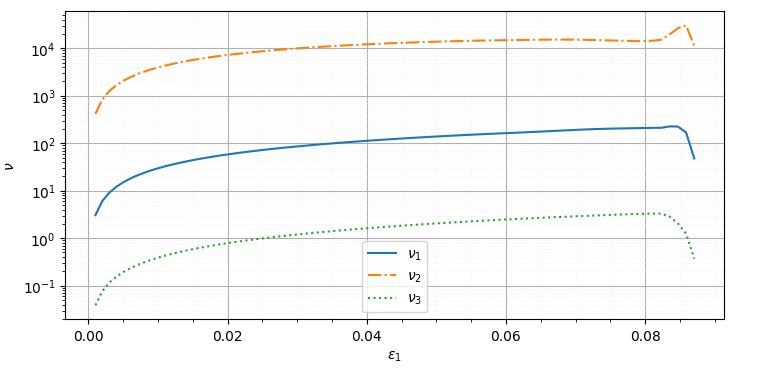
\includegraphics[scale=1.35]{images/mult_soft_nu_eps.JPG}
	}
	\caption{Верхняя граница радиусов неопределённости $\nu_i$, когда $\nu$ не ограничено для задачи \eqref{eq:thm4_OCP}; графики построены относительно значения свободного параметра $\epsilon_1$; вертикальная ось масштабирована логарифмически, обе оси без единиц.}\label{fig:mult_soft_nu}
\end{figure} 
Сначала, решаем оптимизационную задачу \eqref{eq:thm4_OCP} для различных значений $\epsilon_1$ для мягкой мультипликативной неопределённости. 
На рисунке~\ref{fig:mult_soft_nu} показано, как наибольший радиус неопределённости $\nu$, который может выдержать регулятор, зависит от параметра $\epsilon_1$ (показан сплошной синей линией). График вогнутый, и появляется чётко определённое оптимальное решение. На этом же рисунке показан график, построенный при наложении условия \eqref{eq:mu_gamma_limit} (показано пунктирной красной линией). Видно, что наибольший радиус неопределённости ограничивается значением 1.

На рисунке \ref{fig:mult_soft_less_than_unit} ограничим мягкую неопределённость 1.
\begin{figure}[ht]
	\centerfloat{
		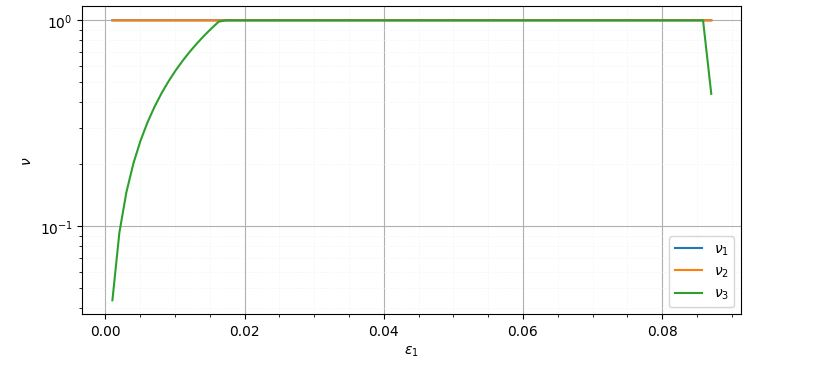
\includegraphics[scale=1.35]{images/mult_soft_less_than_unit.JPG}
	}
	\caption{Верхняя граница радиусов неопределённости $\nu_i$, когда $\nu$ не ограничено для задачи \eqref{eq:thm4_OCP} с целевой функцией \eqref{eq:cost_lin}; графики построены относительно значения свободного параметра $\epsilon_1$; вертикальная ось масштабирована логарифмически, обе оси без единиц.}\label{fig:mult_soft_less_than_unit}
\end{figure}


Затем решим оптимизационную задачу \eqref{eq:thm4_OCP} с квадратичной целевой функцией \eqref{eq:cost_lin}:

\begin{equation}
	\label{eq:thm5_OCP}
	\begin{aligned}
		& \underset{\bar{\mu}_i,\gamma_i, \varpi, {Q}_1, {P}_2,\hat{{K}} , \hat{{L}} }{\text{minimize}}
		& &  \sum_{i=1}^{3}\left((\bar{\mu}_i-\varpi)^2+(\gamma_i-\varpi)^2\right) + \varpi^2, \\
		& \text{subject to}
		& & \begin{cases}
			{Q}_1>0, \ \
			{P}_2>0, \ \
			\bar{\mu}_i>0, \ \
			\gamma_i>0, \ \
			\text{для} \ \ i=1,2,3; \\
			\text{условия \eqref{eq:thm4_final_LMI}, \eqref{eq:mu_gamma_limit} }.
		\end{cases}
	\end{aligned}
\end{equation} 

\begin{figure}[ht]
	\centerfloat{
		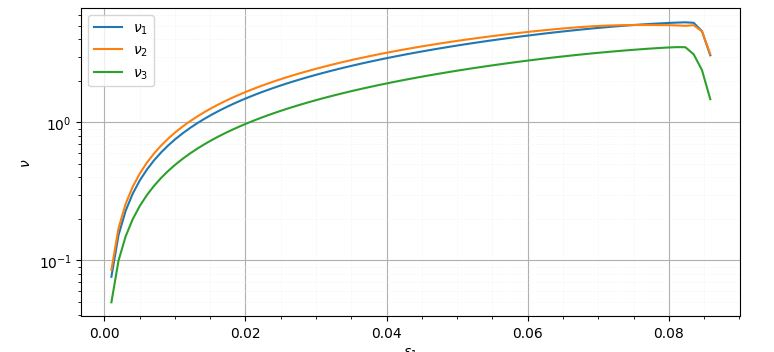
\includegraphics[scale=1.35]{images/mult_soft_nu_eps_qp.JPG}
	}
	\caption{Верхняя граница радиусов неопределённости $\nu_i$, когда $\nu$ не ограничено для задачи \eqref{eq:thm5_OCP}; графики построены относительно значения свободного параметра $\epsilon_1$; вертикальная ось масштабирована логарифмически, обе оси без единиц.}\label{fig:mult_soft_nu_eps_qp}
\end{figure}


\begin{figure}[ht]
	\centerfloat{
		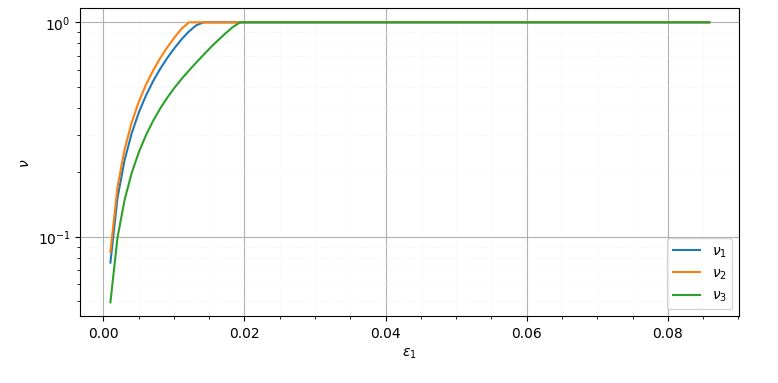
\includegraphics[scale=1.35]{images/mult_soft_less_than_unit_qp.JPG}
	}
	\caption{Верхняя граница радиусов неопределённости $\nu_i$, когда $\nu$ ограничено для задачи \eqref{eq:thm5_OCP}; графики построены относительно значения свободного параметра $\epsilon_1$; вертикальная ось масштабирована логарифмически, обе оси без единиц.}\label{fig:mult_soft_leq_qp}
\end{figure}

На рисунке \ref{fig:mult_soft_leq_qp} показана зависимость радиусов неопределённости от параметра $\epsilon_1$
  
\chapter{Аддитивная неопределённость c динамической обратной связью}\label{ch:ch5}
\section{Динамическая обратная связь}\label{sec:ch5/sect1}
Рассмотрим следующую систему:
\begin{equation}
	\label{eq:part5_linear_dynamics}
	\begin{cases}
		\dot z={A}_n {z} + {A}_r {\zeta} + {B} {u},\\
		y = {C} {N} {z} + {C} {R} {\zeta},
	\end{cases}
\end{equation}
где матрицы $A_n$,  $B$ и $C$ являются матрицами состояния, управления и наблюдения соответственно. А матрица ${A}_r$ отвечает за статическую часть матрицы состояния.

Рассмотрим следующий закон управления с динамической обратной связью:
\begin{equation}
	\label{eq:part5_controller}
	\begin{cases}
		\dot{{z}}_K = {A}_K {z}_K + {B}_K {y},\\
		{u} = {C}_K {z}_K + {D}_K {y}.
	\end{cases}
\end{equation}
Мы можем переписать предыдущую систему уравнений как:
\begin{align}
	\label{eq:part5_system1}
	&\begin{bmatrix}
		{\dot{z}} \\ {\dot{z}}_K
	\end{bmatrix}
	=
	\begin{bmatrix}
		{A}_N & 0 \\
		0 & {A}_K
	\end{bmatrix}
	\begin{bmatrix}
		{z} \\ {z}_K 
	\end{bmatrix}
	+
	\begin{bmatrix}
		{B} & 0 \\
		0 & {B}_K 
	\end{bmatrix}
	\begin{bmatrix}
		{u} \\ {y}
	\end{bmatrix}
	+
	\begin{bmatrix}
		{A}_R \\ 0 
	\end{bmatrix}
	\zeta,
	\\
	\label{eq:part5_system2}
	& \begin{bmatrix}
		{I} & -{D}_K \\
		0 & {I}
	\end{bmatrix}
	\begin{bmatrix}
		{u} \\ {y}
	\end{bmatrix}
	=
	\begin{bmatrix}
		0 & {C}_K \\
		{C} {N} & 0
	\end{bmatrix}
	\begin{bmatrix}
		{z} \\ {z}_K
	\end{bmatrix}
	+
	\begin{bmatrix}
		0 \\ {C} {R}
	\end{bmatrix}{\zeta},
\end{align}
где матрица $\bigl[ \begin{smallmatrix}  {I} & -{D}_K \\ 0 & {I} \end{smallmatrix} \bigr]$ должна быть невырожденной, которая она и будет всегда являться, следуя:
\begin{equation}
	\begin{gathered}
		\begin{bmatrix}
			{I} & -{D}_K \\ 0 & {I}
		\end{bmatrix}^{-1} = 
		\\
		=\begin{bmatrix}
			{I} + {I}(-{D}_K)({I}-0*{I}(-{D}_K))*0*{I} & -{I}(-{D}_K)({I}-0*{I}(-{D}_K))^{-1}\\
			-({I} - 0*{I}({D}_K))^{-1}*0*{I} &
			{I}-(0*{I}(-{D}_K))^{-1}
		\end{bmatrix}= \\
		=
		\begin{bmatrix}
			{I} & {D}_K \\ 0 & {I}
		\end{bmatrix}.
	\end{gathered}
\end{equation}
Подставим \eqref{eq:part5_system2} в \eqref{eq:part5_system1}:
\begin{align}
	\nonumber
	& \begin{bmatrix}
		{\dot{z}} \\ {\dot{z}}_K 
	\end{bmatrix}
	=\left(
	\begin{bmatrix}
		{A}_N & 0 \\
		0 & {A}_K
	\end{bmatrix}
	+
	\begin{bmatrix}
		{B} & 0 \\
		0 & {B}_K
	\end{bmatrix}
	\begin{bmatrix}
		{I} & {D}_K \\
		0 & {I}
	\end{bmatrix}
	\begin{bmatrix}
		0 & {C}_K \\
		{C}{N} & 0
	\end{bmatrix}
	\right)
	\begin{bmatrix}
		{z} \\ {z}_K
	\end{bmatrix}
	+ \\
	& + \left(
	\begin{bmatrix}
		{B} & 0 \\
		0 & {B}_K
	\end{bmatrix}
	\begin{bmatrix}
		{I} & {D}_K \\
		0 & {I}
	\end{bmatrix}
	\begin{bmatrix}
		0 \\ {C}{R}
	\end{bmatrix}
	+
	\begin{bmatrix}
		{A}_R \\ 0 
	\end{bmatrix}\right)
	{\zeta}.
\end{align}
Раскроем скобки и упростим выражение:
\begin{align}
	\label{eq:part5_cl}
	&\begin{bmatrix}
		{\dot{z}} \\ {\dot{z}}_K 
	\end{bmatrix}
	=
	\begin{bmatrix}
		{A}_N + {B}{D}_K{C}{N} & {B}{C}_K \\
		{B}_K{C}{N} &{A}_K
	\end{bmatrix}
	\begin{bmatrix}
		{z} \\ {z}_K 
	\end{bmatrix}
	+
	\begin{bmatrix}
		{A}_R + {B}{D}_K{C}{R}\\ {B}_K{C}_R
	\end{bmatrix}
	{\zeta}.
\end{align}
Обозначим:
\begin{align}
	{A}_{cl} = \begin{bmatrix}
		{A}_N + {B}{D}_K{C}{N} & {B}{C}_K \\
		{B}_K{C}{N} & {A}_K
	\end{bmatrix},
	\quad
	{z}_{cl} = \begin{bmatrix}
		{\dot{z}} \\ {\dot{z}}_K 
	\end{bmatrix},
	\quad
	{F}_{cl} = \begin{bmatrix}
		{A}_R + {B}{D}_K{C}{R}\\ {B}_K{C}_R
	\end{bmatrix}.
\end{align}
Используя новые обозначения, перепишем \eqref{eq:part5_cl}, как:
\begin{align}
	\label{eq:part5_system}
	&{\dot{z}}_{cl} = {A}_{cl} {z}_{cl}+ {F}_{cl}\zeta.
\end{align}
\begin{theorem}
	Система \eqref{eq:part5_system} асимптотически устойчива, если существуют положительно-определённые матрицы ${Q}_1>0$, ${P}_1>0$, матрицы $\hat{{A}}_K$,  $\hat{{B}}_K$, $\hat{{C}}_K$ и $D_K$
	и положительный скаляр $\alpha>0$ такие, что выполняется следующие линейные матричные неравенства:
		\begin{align}\label{eq:part5_finalLMI}
		\begin{bmatrix}
			{\Theta}_1  & {A}_N + {\hat{A}}_K\T +{B}{D}_K{C}{N} & {A}_R + {B}{D}_K{C}{R}\\
			\cdots & {\Theta}_2 & {P}_{1}{A}_R + {P}_{1}{B}{D}_K{C}{R}+{P}_1{B}_K{C}{R}\\
			\cdots & \cdots & 0 
		\end{bmatrix} < 
		\begin{bmatrix}
			0 & 0\\
			0 & \alpha {I}
		\end{bmatrix},
	\end{align}
	где
	\begin{align}
		{\Theta}_1 = {A}_N{Q}_{1} +{Q}_{1}{A}_N\T + {B}{\hat{C}}_K +{\hat{C}}_K\T{B}\T, \\
		{\Theta}_2 = {P}_{1}{A}_N +{A}_N\T{P}_{1}+{\hat{B}}_K{C}{N}+{N}\T{C}\T{\hat{B}}_K\T.
	\end{align}
	И
	\begin{align}\label{eq: condition}
		\begin{bmatrix} 
			{Q}_{1} & I \\ 
			I & {P}_{1}
		\end{bmatrix} > 0.
	\end{align}
	И коэффициенты регулятора находятся следующим образом 
	\begin{align}
		&{P}_{2} = ({I}-{P}_{1}{Q}_{1})({Q}_{2}\T)^{-1},\\
		&{C}_K = ({\hat{C}}_K - {D}_K {C} {N} {Q}_{1} ) ({Q}_{2}\T)^{-1},\\
		&{B}_K = {P}_{2}^{-1}({\hat{B}}_K- {P}_{1}{B}{D}_K),\\
		&{A}_K = {P}_{2}^{-1}({\hat{A}}_K-{P}_{1}({A}_N+{B}{D}_K{C}{N}){Q}_{1} - {P}_{2}{B}_K{C}{C}{Q}_{1}-{P}_{1} {B}{C}_K{Q}_{2}\T)({Q}_{2}\T)^{-1}.
	\end{align}
\end{theorem}
\begin{proof}
	Введём кандидата в функцию Ляпунова ${V} = {z}_{cl}\T {P}{z}_{cl} > 0$ и её производную:
	\begin{align}
		{\dot{V}} = {z}_{cl}\T {P} {A}_{cl} {z}_{cl} +
		{z}_{cl}\T {A}_{cl}\T {z}_{cl} 
		+
		{z}_{cl}\T {P} {F}_{cl} {\zeta} +
		{\zeta}\T {F}_{cl}\T {z}_{cl}
		< 0,
	\end{align}
	где система считается асимптотически устойчивой в конечное время тогда и только тогда, когда существует положительно--определённая матрица ${P} = \bigl[ \begin{smallmatrix}  {P}_1 & {P}_2 \\ {P}_2\T & {P}_3 \end{smallmatrix} \bigr]$.
	Производная от кандидата в функции Ляпунова может быть переписана как:
		\begin{align}
			\begin{bmatrix}
				z_cl \\ \zeta
			\end{bmatrix}\T
		\begin{bmatrix}
			{P} {A}_{cl} + {A}_{cl}\T {P} & {P} {F}_{cl} \\
			{F}_{cl} \T {P} & 0
		\end{bmatrix} 
		\begin{bmatrix}
			z_cl & \zeta
		\end{bmatrix} < 0.
	\end{align}
	Перепишем как
	\begin{align}
		\begin{bmatrix}
			{P} {A}_{cl} + {A}_{cl}\T {P} & {P} {F}_{cl} \\
			{F}_{cl} \T {P} & 0
		\end{bmatrix} < 0.
	\end{align}
	Введём релаксацию, добавляя параметр $\alpha$, который и будет условием релаксации:
	\begin{align}\label{eq: S procedure}
		\begin{bmatrix}
			{P} {A}_{cl} + {A}_{cl}\T {P} & {P} {F}_{cl} \\
			{F}_{cl} \T {P} & 0
		\end{bmatrix} < 
		\begin{bmatrix}
			0 & 0\\
			0 & \alpha {I}
		\end{bmatrix}.
	\end{align}
	Далее нам необходимо избавиться от нелинейности в переменных и для этого вводим следующую лемму:
	\begin{lemma}
		Даны симметричные и невырожденные матрицы ${Q}_{1} \in \mathbb{R}^{n\times n}$ и ${P}_{1} \in \mathbb{R}^{n\times n}$. Следующие утверждения эквивалентны.\\
		
		i). Существуют симметричные и невырожденные матрицы  ${P}_{3}$ и ${Q}_{3} \in \mathbb{R}^{m\times m}$ и матрицы с полным рангом ${P}_{2}$ и ${Q}_{2} \in \mathbb{R}^{n\times m}$ такие, что
		
		\begin{align*}
			{P}=
			\begin{bmatrix} 
				{P}_{1} & {P}_{2}\\ 
				{P}_{2}\T & {P}_{3} 
			\end{bmatrix} =
			\begin{bmatrix} 
				{Q}_{1} & {Q}_{2} \\ 
				{Q}_{2}\T & {Q}_{3}
			\end{bmatrix}^{-1}={Q}^{-1}>0,
		\end{align*} 
		где ${Q}_{CL}=
		\begin{bmatrix} 
			{Q}_{1} & {I} \\ {Q}_{2}\T & 0
		\end{bmatrix}$ является матрицей полного ранга.\\
		
		ii). \begin{align*}
			\begin{bmatrix} 
				{Q}_{1} & I \\ 
				I & {P}_{1}
			\end{bmatrix} > 0.
		\end{align*}
	\end{lemma}
	\begin{proof}
		Из i)., берём 
		\begin{align}
			&{P} = {Q}^{-1},\\
			&{P}{Q}={I},\\
			&\begin{bmatrix} 
				{P}_{1} & {P}_{2}\\ 
				{P}_{2}\T & {P}_{3} 
			\end{bmatrix}
			\begin{bmatrix} 
				{Q}_{1} & {Q}_{2} \\ 
				{Q}_{2}\T & {Q}_{3}
			\end{bmatrix} = 
			\begin{bmatrix}
				{I} & 0 \\
				0 & {I}
			\end{bmatrix}.
		\end{align}
		Раскрыв скобки в последнем уравнении, мы получаем:
		\begin{align}
			&{P}_{1}{Q}_{1}+{P}_{2}{Q}_{2}\T ={I},\\
			&{P}_{1}\T{Q}_{2}+{P}_{2}{Q}_{3} =0\label{eq: lemma mult1},\\
			&{P}_{2}\T{Q}_{1}+{P}_{3}{Q}_{2}\T=0,\\
			&{P}_{2}\T{Q}_{2}+{P}_{3}{Q}_{3}= {I} \label{eq: lemma mult2}.
		\end{align}
		Из данных уравнений мы получаем:
		\begin{align}
			{P}{Q}_{CL}={P}_{CL},
		\end{align}
		где
		\begin{align}
			{Q}_{CL}=
			\begin{bmatrix}
				{Q}_{1} & {I}\\
				{Q}_{2}\T & 0
			\end{bmatrix},\\
			{P}_{CL}=
			\begin{bmatrix}
				{I} & {P}_{1} \\
				0 & {P}_{2}\T
			\end{bmatrix}.
		\end{align}
		Матрица ${Q}_{2}$ имеет полный ранг, и матрица ${Q}_{CL}$ тоже имеет полный ранг, тогда
		\begin{align}
			0<{Q}_{CL}\T {P} {Q}_{CL} = {Q}_{CL}\T {P}_{CL} = 
			\begin{bmatrix} 
				{Q}_{1} & I \\ 
				I & {P}_{1}
			\end{bmatrix}.
		\end{align}
		
		И наоборот, предположим ii). верно. Мы можем умножить на $-1$ и применить дополнение Шура к неравенству 
		$\bigl( \begin{smallmatrix} 
			{Q}_{1} & I \\ 
			I & {P}_{1}\end{smallmatrix} \bigr) <0$. 
		И тогда, согласно дополнению Шура, получаем $-{P}_{1}<0$ и $-{Q}_{1}-(-{I})(-{P}_{1})^{-1}(-{I})\T<0$. Упрощая, избавляясь от матриц тождества, мы получаем ${P}_{1}^{-1}-{Q}_{1}<0$, и она имеет полный ранг, то есть можно найти обратную матрицу. Что также означает, что ${I}-{P}_{1}{Q}_{1}$ имеет обратную матрицу.\\\
		
		Выбираем любые две матрицы полного ранга ${P}_{2}$ и ${Q}_{2}$, такие что ${P}_{2}{Q}_{2}\T={I}-{P}_{1}{Q}_{1}$. И поскольку ${P}_2$ и ${Q}_2$ имеют полный ранг, ${Q}_{CL}=\bigl[\begin{smallmatrix}  
			{Q}_{1} & {I}\\
			{Q}_{2}\T & 0
		\end{smallmatrix} \bigr]$ и 
		${P}_{CL}=\bigl[ \begin{smallmatrix}
			{I} & {P}_{1} \\
			0 & {P}_{2}\T
		\end{smallmatrix} \bigr]$ также имеют полный ранг и существуют обратные матрицы к ним.\\
		
		Обозначим ${P}$ и ${Q}$ как 
		\begin{align*}
			{P} = {P}_{CL}{Q}_{CL}^{-1}, \qquad {Q} ={Q}_{CL}{P}_{CL}^{-1}.
		\end{align*} 
		Далее перемножая ${P}$ и ${Q}$, мы получаем единичную матрицу
		\begin{align*}
			{P}{Q}={P}_{CL}{Q}_{CL}^{-1}{Q}_{CL}{P}_{CL}^{-1}={I}.
		\end{align*}
		Таким образом ${P}={Q}^{-1}$.
		
		${P}_3$ и ${Q}_3$ при необходимости можно найти из \eqref{eq: lemma mult1}-\eqref{eq: lemma mult2}.
	\end{proof}
	Домножим с правой и левой стороны правую часть (\ref{eq: S procedure}) на матрицы $diag({Q}_{CL}\T, {I}, {I})$ и $diag({Q}_{CL}, {I}, {I})$ для линеаризации неравенств в переменных:
	\begin{align}
		\begin{bmatrix}
			{Q}_{CL}\T{A}_{CL}\T {P}_{CL} + {P}_{CL}\T{A}_{CL}{Q}_{CL} & {P}_{CL}\T{F}_{CL} \\
			{F}_{CL}\T{P}_{CL} & 0
		\end{bmatrix} < 
		\begin{bmatrix}
			0 & 0\\
			0 & \alpha {I}
		\end{bmatrix}.
	\end{align}
	Далее мы постепенно раскрываем и упрощаем каждый компонент уравнения
	\begin{align}
		{P}_{CL}\T{F}_{CL} = \begin{bmatrix}
			{I} & 0 \\
			{P}_{1} & {P}_{2}
		\end{bmatrix}
		\begin{bmatrix}
			{A}_R + {B}{D}_K{C}{R}\\ {B}_K{C}_R
		\end{bmatrix} =
		\begin{bmatrix}
			{A}_R + {B}{D}_K{C}{R}\\
			{P}_{1}{A}_R + {P}_{1}{B}{D}_K{C}{R}+{P}_1{B}_K{C}{R}
		\end{bmatrix},
	\end{align}
	%
	\begin{align}
		&{Q}_{CL}\T{A}_{CL}\T {P}_{CL} + {P}_{CL}\T{A}_{CL}{Q}_{CL} = \nonumber \\
		& = \begin{bmatrix}
			{A}_N{Q}_{1} +{Q}_{1}{A}_N\T + {B}{\hat{C}}_K +{\hat{C}}_K\T{B}\T & {A}_N + {\hat{A}}_K\T +{B}{D}_K{C}{N}\\
			{A}_N\T + {N}\T{C}\T{D}_K\T{B}\T+{\hat{A}}_K & {P}_{1}{A}_N +{A}_N\T{P}_{1}+{\hat{B}}_K{C}{N}+{N}\T{C}\T{\hat{B}}_K\T
		\end{bmatrix},   
	\end{align}
	\begin{align}
		&{\hat{C}}_K= {D}_K{C}{N}{Q}_{1} + {C}_K{Q}_{2}\T,\\
		&{\hat{B}}_K = {P}_{1}{B}{D}_K + {P}_{2}{B}_K,\\
		&{\hat{A}}_K = {P}_{1}({A}_N+{B}{D}_K{C}{N}){Q}_{1}+{P}_{2}{B}_K{C}{N}{Q}_{1}+{P}_{1}{B}{C}_K{Q}_{2}\T+{P}_{2}{A}_K{Q}_{2}\T.
	\end{align}
	Финальное неравенство
	\begin{align}\label{eq: final LMI}
		\begin{bmatrix}
			{\Theta}_1  & {A}_N + {\hat{A}}_K\T +{B}{D}_K{C}{N} & {A}_R + {B}{D}_K{C}{R}\\
			\cdots & {\Theta}_2 & {P}_{1}{A}_R + {P}_{1}{B}{D}_K{C}{R}+{P}_1{B}_K{C}{R}\\
			\cdots & \cdots & 0 
		\end{bmatrix} < 
		\begin{bmatrix}
			0 & 0\\
			0 & \alpha {I}
		\end{bmatrix},
	\end{align}
	где
	\begin{align}
		&{\Theta}_1 = {A}_N{Q}_{1} +{Q}_{1}{A}_N\T + {B}{\hat{C}}_K +{\hat{C}}_K\T{B}\T, \\
		&{\Theta}_2 = {P}_{1}{A}_N +{A}_N\T{P}_{1}+{\hat{B}}_K{C}{N}+{N}\T{C}\T{\hat{B}}_K\T.
	\end{align}
	И держится неравенство: 
	\begin{align}\label{eq: condition}
		\begin{bmatrix} 
			{Q}_{1} & I \\ 
			I & {P}_{1}
		\end{bmatrix} > 0.
	\end{align}
	Это и является линейным матричным неравенством с переменными ${Q}_1,{P}_1, {\hat{A}}_K, {\hat{B}}_K,{\hat{C}}_K, {D}_K$ и $\alpha$.
\end{proof}
Целевой функцией будет являться минимизация параметра  $\alpha$ (добавить почему). Оптимизационная задача будет выглядеть следующим образом:
%
\begin{equation}
	\label{eq:thm2_OCP}
	\begin{aligned}
		& \underset{{Q}_1,{P}_1, {\hat{A}}_K, {\hat{B}}_K,{\hat{C}}_K, {D}_K, \alpha }{\text{минимизируя}}
		& &  \alpha, \\
		& \text{при ограничениях}
		& & \begin{cases}
			\text{условия \eqref{eq: final LMI}, \eqref{eq: condition}}.
		\end{cases}
	\end{aligned}
\end{equation}

\section{Эксперименты}\label{sec:ch5/sect2}
\subsection{Параметры эксперимента}\label{sec:ch5/sect2/sub1}
Используем математическую модель шагающего робота ту же что и в предыдущих главах.
\subsection{Результаты эксперимента}\label{sec:ch5/sect2/sub2}           % Глава 3
\chapter*{Заключение}                       % Заголовок
\addcontentsline{toc}{chapter}{Заключение}  % Добавляем его в оглавление

%% Согласно ГОСТ Р 7.0.11-2011:
%% 5.3.3 В заключении диссертации излагают итоги выполненного исследования, рекомендации, перспективы дальнейшей разработки темы.
%% 9.2.3 В заключении автореферата диссертации излагают итоги данного исследования, рекомендации и перспективы дальнейшей разработки темы.
%% Поэтому имеет смысл сделать эту часть общей и загрузить из одного файла в автореферат и в диссертацию:

Основные результаты работы заключаются в следующем:
%% Согласно ГОСТ Р 7.0.11-2011:
%% 5.3.3 В заключении диссертации излагают итоги выполненного исследования, рекомендации, перспективы дальнейшей разработки темы.
%% 9.2.3 В заключении автореферата диссертации излагают итоги данного исследования, рекомендации и перспективы дальнейшей разработки темы.
\begin{enumerate}
  \item В результате анализа научных публикаций, установлено, что имеющиеся методы основанные на линейных матричных неравенствах не обладают достаточной робастностью, так как не учитывают неопределённости одновременно во всех матрицах. Исходя из этого предложен новый метод построения линейных матричных неравенств для систем с мультипликативными неопределённостями и ортогональной декомпозиции.  
  \item Предложено прямой и обратной динамики шагающих роботов и описаны используемые в работе математические инструменты.
  \item Разработан метод нахождения оптимального робастного управления для систем с мультипликативной неопределённостью и в матрицах состояния, управления и наблюдения. 
  \item разработан метод обобщающий предыдущий, где неопределённости не ограничены единичной матрицей, а находится наибольшие возможные неопределённости для стабилизации системы.
  \item Разработан метод нахождения оптимального робастного управления для систем с мультипликативной и аддитивной неопределённостью. Рассмотрены случаи для единичной и мягкой неопределённостей.
  \item Разработан метод нахождения оптимального робастного управления для систем с аддитивной неопределённостью и динамической обратной связью.
  \item Численные исследования показали, что разработанные методы выполняют обозначенную функцию нахождения оптимального робастного управления с помощью линейных матричных неравенств.
  \item Математическое моделирование показало, что предложенные методы могут быть применены для управления четвероногими шагающими роботами. 
\end{enumerate}


В настоящее время использование линейных матричных неравенств для нахождения оптимального робастного управления является развивающимся направлением для исследований так как они предоставляют математические гарантии устойчивости. И применение разработанных методов может расширить границы применения шагающих роботов, делая системы более устойчивыми к неопределённостям.  
      % Заключение
\include{Dissertation/acronyms}        % Список сокращений и условных обозначений
\chapter*{Словарь терминов}             % Заголовок
\addcontentsline{toc}{chapter}{Словарь терминов}  % Добавляем его в оглавление

\textbf{\(H_\infty\)} : Cистема компьютерной вёрстки, разработанная американским профессором информатики Дональдом Кнутом

\textbf{\(L_2\)} : норма, является геометрическим расстоянием между двумя точками в многомерном пространстве, вычисляемым по теореме Пифагора

\textbf{Позитивно определённая матрица}
      % Словарь терминов
\clearpage                                  % В том числе гарантирует, что список литературы в оглавлении будет с правильным номером страницы
%\hypersetup{ urlcolor=black }               % Ссылки делаем чёрными
%\providecommand*{\BibDash}{}                % В стилях ugost2008 отключаем использование тире как разделителя
\urlstyle{rm}                               % ссылки URL обычным шрифтом
\ifdefmacro{\microtypesetup}{\microtypesetup{protrusion=false}}{} % не рекомендуется применять пакет микротипографики к автоматически генерируемому списку литературы
\insertbibliofull                           % Подключаем Bib-базы: все статьи единым списком
% Режим с подсписками
%\insertbiblioexternal                      % Подключаем Bib-базы: статьи, не являющиеся статьями автора по теме диссертации
% Для вывода выберите и расскомментируйте одно из двух
\insertbiblioauthor                        % Подключаем Bib-базы: работы автора единым списком 
%\insertbiblioauthorgrouped                 % Подключаем Bib-базы: работы автора сгруппированные (ВАК, WoS, Scopus и т.д.)
\ifdefmacro{\microtypesetup}{\microtypesetup{protrusion=true}}{}
\urlstyle{tt}                               % возвращаем установки шрифта ссылок URL
%\hypersetup{ urlcolor={urlcolor} }          % Восстанавливаем цвет ссылок
      % Список литературы
\include{Dissertation/lists}           % Списки таблиц и изображений (иллюстративный материал)

\setcounter{totalchapter}{\value{chapter}} % Подсчёт количества глав

%%% Настройки для приложений
\appendix
% Оформление заголовков приложений ближе к ГОСТ:
\setlength{\midchapskip}{20pt}
\renewcommand*{\afterchapternum}{\par\nobreak\vskip \midchapskip}
\renewcommand\thechapter{\Asbuk{chapter}} % Чтобы приложения русскими буквами нумеровались

\chapter{Доказательство}\label{app:A}
\begin{comment}
Выражение \eqref{eq:Young_conjugated} может быть записано как:
%
\begin{multline}
	\begin{bmatrix}
		{\Pi}_1 & 0 \\ 0 & {\Sigma}_2 
	\end{bmatrix}+
	\begin{bmatrix}
		0&-{BK}\\-({BK})\T&0
	\end{bmatrix}+
	\begin{bmatrix}
		{M}_1{F}_1{N}_1{Q}_1 + {Q}_1({M}_1{F}_1{N}_1)\T&0 \\ 0& 0
	\end{bmatrix}
	\\ + \begin{bmatrix}
		0& {Q}_1({S} {M}_1{F}_1{N}_1)\T{P}_2 \\
		{P}_2{M}_1{F}_1{N}_1{Q}_1 - ({BK})\T & 0
	\end{bmatrix}<0,
\end{multline}
%
раскрываем:
%
\begin{multline}
	\label{eq:Young_expand}
	\begin{bmatrix}
		{\Pi}_1 & 0 \\ 0 & {\Sigma}_2 
	\end{bmatrix}+ \begin{bmatrix}
		-{BK} \\ 0
	\end{bmatrix}\begin{bmatrix}
		0 \\ {I}
	\end{bmatrix}\T
	+\begin{bmatrix}
		0 \\ {I} 
	\end{bmatrix}\begin{bmatrix}
		-{BK} \\0
	\end{bmatrix}\T+\begin{bmatrix}
		{Q}_1{N}_1\T \\0
	\end{bmatrix}{F}_1\T\begin{bmatrix}
		{M}_1 \\0
	\end{bmatrix}\T \\ + \begin{bmatrix}
		{M}_1 \\0
	\end{bmatrix}{F}_1\begin{bmatrix}
		{Q}_1{N}_1\T \\0
	\end{bmatrix}\T+\begin{bmatrix}
		{Q}_1{N}_1\T \\ 0
	\end{bmatrix}{F}_1\T\begin{bmatrix}
		0 \\ {P}_2{S}{M}_1
	\end{bmatrix}\T+  \begin{bmatrix}
		0\\ {P}_2{S}{M}_1
	\end{bmatrix}{F}_1\begin{bmatrix}
		{Q}_1{N}_1\T \\0
	\end{bmatrix}\T<0.
\end{multline}
%
Используя \eqref{eq:Young_relation_BMI} из леммы \ref{lemma:Young} \cite{KHELOUFI2013}, находим:
%
\begin{multline}
	\label{eq:thm1_term_1}
	\begin{bmatrix}
		-{BK} \\ 0
	\end{bmatrix}\begin{bmatrix}
		0 \\ {I}
	\end{bmatrix}\T
	+\begin{bmatrix}
		0 \\ {I} 
	\end{bmatrix}\begin{bmatrix}
		-{BK} \\0
	\end{bmatrix}\T 
	\\ 
	\leq
	\begin{bmatrix}
		-{BK} \\ 0
	\end{bmatrix} \epsilon_1 {H} \begin{bmatrix}
		-{BK} \\ 0
	\end{bmatrix}\T +\begin{bmatrix}
		0 \\ {I}
	\end{bmatrix}\frac{1}{\epsilon_1}{H}^{-1}\begin{bmatrix}
		0 \\ {I}
	\end{bmatrix}\T =
	\begin{bmatrix}
		{BK}\epsilon_1{H}{K}\T{B}\T & 0 \\
		0 & \frac{1}{\epsilon_1}{H}^{-1}
	\end{bmatrix}.
\end{multline}
%
Из неравенства \eqref{eq:Young_robust_2} и леммы \ref{lemma:Young} с $\nu=1$ получаем:
%
\begin{multline}
	\label{eq:thm1_term_2}
	\begin{bmatrix}
		{Q}_1{N}_1\T \\0
	\end{bmatrix}{F}_1\T\begin{bmatrix}
		{M}_1 \\0
	\end{bmatrix}\T+\begin{bmatrix}
		{M}_1 \\0
	\end{bmatrix}{F}_1\begin{bmatrix}
		{Q}_1{N}_1\T \\0
	\end{bmatrix}\T  \\ \leq \frac{1}{\epsilon_2}\begin{bmatrix}
		{Q}_1{N}_1\T \\0
	\end{bmatrix}\begin{bmatrix}
		{Q}_1{N}_1\T \\ 0
	\end{bmatrix}\T +\epsilon_2 \begin{bmatrix}
		{M}_1 \\0
	\end{bmatrix}\begin{bmatrix}
		{M}_1 \\0
	\end{bmatrix}\T.
\end{multline}
%
Похожим образом:
%
\begin{multline}
	\label{eq:thm1_term_3}
	\begin{bmatrix}
		{Q}_1{N}_1\T \\0
	\end{bmatrix}{F}_1\T\begin{bmatrix}
		0 \\ {P}_2{S}{M}_1
	\end{bmatrix}\T+\begin{bmatrix}
		0\\ {P}_2{S}{M}_1
	\end{bmatrix}{F}_1\begin{bmatrix}
		{Q}_1{N}_1\T \\0
	\end{bmatrix}\T \\ \leq  \frac{1}{\epsilon_3}\begin{bmatrix}
		{Q}_1{N}_1\T \\0
	\end{bmatrix}\begin{bmatrix}
		{Q}_1{N}_1\T \\ 0
	\end{bmatrix}\T +\epsilon_3 \begin{bmatrix}
		0 \\ {P}_2{S}{M}_1
	\end{bmatrix}\begin{bmatrix}
		0 \\ {P}_2{S}{M}_1
	\end{bmatrix}\T.
\end{multline}
%
Подставляя \eqref{eq:thm1_term_1},\eqref{eq:thm1_term_2} и \eqref{eq:thm1_term_3} в \eqref{eq:Young_expand} получаем выражение \eqref{eq:thm1_LMI_after_Young}.

\clearpage
\refstepcounter{chapter}

\end{comment}
CVXPY - это встроенный в Python язык моделирования выпуклых оптимизационных задач с открытым исходным кодом. Он позволяет выразить задачу естественным образом, следуя математике, а не в ограничительной стандартной форме, требуемой решателями.        % Приложения

\setcounter{totalappendix}{\value{chapter}} % Подсчёт количества приложений

\end{document}
